% !TeX program = xelatex
\documentclass[11pt]{article}
\usepackage[a4paper,margin=25mm]{geometry}
\usepackage{fontspec,libertine,amsmath,amssymb,amsthm,booktabs,array,longtable,graphicx}
\usepackage[ruled,vlined,linesnumbered]{algorithm2e}
\usepackage{placeins,needspace,xurl,tikz}
\setlength{\emergencystretch}{2em}
\usetikzlibrary{automata,positioning,arrows.meta,fpu}
\providecommand{\Description}[1]{}
\usepackage[numbers]{natbib}
\usepackage{xr-hyper}
\usepackage[hidelinks]{hyperref}
\externaldocument{build/main}[main.pdf]
\hypersetup{pdftitle={Technical Appendix: Controller-Preserving Update Synthesis},pdfauthor={Anonymous Authors}}
\newtheorem{lemma}{Lemma}[section]
\newtheorem{theorem}[lemma]{Theorem}
\newtheorem{proposition}[lemma]{Proposition}
\renewcommand{\thetable}{A\arabic{table}}
\renewcommand{\thefigure}{A\arabic{figure}}
\newcommand{\Post}{\mathsf{Post}}
\newcommand{\Safe}{\mathsf{Safe}}
\newcommand{\Goal}{Q_{\mathrm{goal}}}
\newcommand{\rank}{\mathsf{rk}}
\newcommand{\ActT}{\mathsf{ActiveM}}
\newcommand{\Init}{\mathsf{Init}}
\newcommand{\Reach}{\mathsf{Reach}}
\newcommand{\SuccSet}{\mathsf{Succ}}
\newcommand{\En}{\mathsf{En}}
\newcommand{\Cand}{\mathsf{Next}}
\newcommand{\Sigmauc}{\Sigma_{\mathrm{uc}}}
\newcommand{\Sigmac}{\Sigma_{\mathrm{c}}}
\newcommand{\SigmaN}{\Sigma_{\mathrm{N}}}
\newcommand{\SigmaU}{\Sigma_{\mathrm{upd}}}
\newcommand{\CLnew}{\mathsf{CL}^{\mathrm{new}}}
\newcommand{\ustart}[1]{\mathsf{start}(#1)}
\newcommand{\ustop}[1]{\mathsf{stop}(#1)}

% Derived from validated returned raw; elapsed/RSS are single-trial references, not medians.
\providecommand{\ADDirectFullWins}{14}
\providecommand{\ADDirectFullTimeouts}{13}
\providecommand{\ADWorkflowCapSeconds}{1200}
\providecommand{\ADWorkflowElapsedSeconds}{1201.7}
\providecommand{\ADWorkflowPeakRSSGiB}{13.9}
\providecommand{\ADPCCapSeconds}{3600}
\providecommand{\ADPCElapsedSeconds}{3605.2}
\providecommand{\ADPCPeakRSSGiB}{67.1}

% Generated from validated Xeon raw; do not edit.
\newcommand{\LFConditions}{21}
\newcommand{\LFFamilies}{8}
\newcommand{\LFPublishedWins}{21}
\newcommand{\LFForkWins}{16}
\newcommand{\LFSizeMatches}{15}
\newcommand{\LFSizeMismatches}{1}
\newcommand{\LFUnmeasured}{5}
\newcommand{\LFParserNM}{3}
\newcommand{\LFInstrumentationNM}{2}
\newcommand{\LFRailcabStateDelta}{5}
\newcommand{\LFRailcabTransitionDelta}{7}

% Derived elapsed-time bounds, never solver-only bounds.
\newcommand{\CensoredPairs}{12}
\newcommand{\CensoredBoundMin}{2.12}
\newcommand{\CensoredBoundMax}{910.06}

\providecommand{\RSMonitorOccurrences}{273}
\providecommand{\RSClassifiedOccurrences}{273}
\providecommand{\RSFluentDeterminedOccurrences}{0}
\providecommand{\RSExactOccurrences}{0}
\providecommand{\RSUntestedOccurrences}{273}
\providecommand{\RSUnclassifiedOccurrences}{0}
\providecommand{\RSNewOccurrences}{138}
\providecommand{\RSUpdateOccurrences}{135}
\providecommand{\RSAExactOccurrences}{138}
\providecommand{\RSEExactOccurrences}{0}
\providecommand{\RSAEUnverifiedOccurrences}{135}
\providecommand{\RSEObserverSyncOccurrences}{89}
\providecommand{\RSEResetConsistentOccurrences}{135}
\providecommand{\RSEAHExactOccurrences}{89}
\providecommand{\RSAHEUnverifiedOccurrences}{46}
\providecommand{\RSAInclusionNew}{138}
\providecommand{\RSAExactNew}{138}
\providecommand{\RSEExactUpd}{89}
\providecommand{\RSUpdOccurrences}{135}
\providecommand{\RSAUnverifiedNew}{0}
\providecommand{\RSEUnverifiedUpd}{46}

% Generated only from AK saved rq3-cells.csv and rq3-comparisons.csv.
\newcommand{\ApplicationContracts}{27}
\newcommand{\ApplicationModels}{9}
\newcommand{\LazyDecisions}{26}
\newcommand{\EagerDecisions}{17}
\newcommand{\UpdateFirstDecisions}{24}
\newcommand{\DirectFullDecisions}{14}
\newcommand{\UpdateFirstPairs}{24}
\newcommand{\UpdateFirstFaster}{8}

% Generated from saved rq3-cells.csv; native Legacy reference, not a same-game comparator.
% WIN requires five valid identical decisions; N/M counts only CRASH annotated author_capture_cap from saved exception evidence.
\newcommand{\LegacyNativeWins}{9}
\newcommand{\LegacyNativeOOM}{13}
\newcommand{\LegacyCaptureNM}{5}

% Generated from saved xeon-statistics.json; no new measurements.
\newcommand{\TravelSettings}{48}
\newcommand{\TravelOTFDecisions}{20}
\newcommand{\TravelFullDecisions}{18}

% Generated from saved LTS declarations, cross-checked against saved frontend exports.
\providecommand{\ContractGSMComponents}{1}
\providecommand{\ContractGSMTransferPairs}{8}
\providecommand{\ContractGSMUpdates}{3}
\providecommand{\ContractGSMOld}{1}
\providecommand{\ContractGSMNew}{1}
\providecommand{\ContractGSMBase}{0}
\providecommand{\ContractGSMROne}{1}
\providecommand{\ContractGSMRTwo}{2}
\providecommand{\ContractIndustryComponents}{3}
\providecommand{\ContractIndustryTransferPairs}{16}
\providecommand{\ContractIndustryUpdates}{9}
\providecommand{\ContractIndustryOld}{3}
\providecommand{\ContractIndustryNew}{3}
\providecommand{\ContractIndustryBase}{0}
\providecommand{\ContractIndustryROne}{3}
\providecommand{\ContractIndustryRTwo}{6}
\providecommand{\ContractMetaSocketComponents}{2}
\providecommand{\ContractMetaSocketTransferPairs}{3}
\providecommand{\ContractMetaSocketUpdates}{4}
\providecommand{\ContractMetaSocketOld}{1}
\providecommand{\ContractMetaSocketNew}{1}
\providecommand{\ContractMetaSocketBase}{0}
\providecommand{\ContractMetaSocketROne}{1}
\providecommand{\ContractMetaSocketRTwo}{2}
\providecommand{\ContractPowerPlantComponents}{2}
\providecommand{\ContractPowerPlantTransferPairs}{4}
\providecommand{\ContractPowerPlantUpdates}{9}
\providecommand{\ContractPowerPlantOld}{4}
\providecommand{\ContractPowerPlantNew}{3}
\providecommand{\ContractPowerPlantBase}{0}
\providecommand{\ContractPowerPlantROne}{3}
\providecommand{\ContractPowerPlantRTwo}{7}
\providecommand{\ContractPCOneComponents}{1}
\providecommand{\ContractPCOneTransferPairs}{7}
\providecommand{\ContractPCOneUpdates}{13}
\providecommand{\ContractPCOneOld}{6}
\providecommand{\ContractPCOneNew}{6}
\providecommand{\ContractPCOneBase}{0}
\providecommand{\ContractPCOneROne}{6}
\providecommand{\ContractPCOneRTwo}{12}
\providecommand{\ContractPCTwoComponents}{2}
\providecommand{\ContractPCTwoTransferPairs}{14}
\providecommand{\ContractPCTwoUpdates}{26}
\providecommand{\ContractPCTwoOld}{12}
\providecommand{\ContractPCTwoNew}{12}
\providecommand{\ContractPCTwoBase}{0}
\providecommand{\ContractPCTwoROne}{12}
\providecommand{\ContractPCTwoRTwo}{24}
\providecommand{\ContractRailcabComponents}{4}
\providecommand{\ContractRailcabTransferPairs}{11}
\providecommand{\ContractRailcabUpdates}{16}
\providecommand{\ContractRailcabOld}{5}
\providecommand{\ContractRailcabNew}{7}
\providecommand{\ContractRailcabBase}{0}
\providecommand{\ContractRailcabROne}{7}
\providecommand{\ContractRailcabRTwo}{11}
\providecommand{\ContractSurveillanceComponents}{2}
\providecommand{\ContractSurveillanceTransferPairs}{16}
\providecommand{\ContractSurveillanceUpdates}{16}
\providecommand{\ContractSurveillanceOld}{7}
\providecommand{\ContractSurveillanceNew}{7}
\providecommand{\ContractSurveillanceBase}{0}
\providecommand{\ContractSurveillanceROne}{7}
\providecommand{\ContractSurveillanceRTwo}{14}
\providecommand{\ContractWorkflowComponents}{5}
\providecommand{\ContractWorkflowTransferPairs}{12}
\providecommand{\ContractWorkflowUpdates}{16}
\providecommand{\ContractWorkflowOld}{5}
\providecommand{\ContractWorkflowNew}{6}
\providecommand{\ContractWorkflowBase}{0}
\providecommand{\ContractWorkflowROne}{6}
\providecommand{\ContractWorkflowRTwo}{11}

% Generated from extended-budget configs and returned evidence.
\providecommand{\ExtBudgetPlanned}{27}
\providecommand{\ExtBudgetChecked}{8}
\providecommand{\ExtBudgetTimeout}{16}
\providecommand{\ExtBudgetOOM}{1}
\providecommand{\ExtBudgetSkipped}{2}
\providecommand{\ExtBudgetPending}{0}
\providecommand{\ExtBudgetReceived}{27}
\providecommand{\ExtBudgetTimeCap}{7{,}200}
\providecommand{\ExtBudgetInitialHeap}{64}
\providecommand{\ExtBudgetExpandedHeap}{200}
\providecommand{\ExtBudgetWins}{7}
\providecommand{\ExtBudgetLosses}{1}
\providecommand{\ExtTravelFourFourDFSeconds}{1{,}872}
\providecommand{\ExtTravelFourFourDFSolverSeconds}{1{,}814}
\providecommand{\ExtTravelFourFourDFStates}{412{,}688}
\providecommand{\ExtTravelFourFourDFRSS}{7}
\providecommand{\ExtTravelFourSixDFSeconds}{6{,}990}
\providecommand{\ExtTravelFourSixDFSolverSeconds}{6{,}768}
\providecommand{\ExtTravelFourSixDFStates}{817{,}362}
\providecommand{\ExtTravelFourSixDFRSS}{13}
\providecommand{\ExtTravelFourEightLazySeconds}{1{,}636}
\providecommand{\ExtTravelFourEightLazySolverSeconds}{756}
\providecommand{\ExtTravelFourEightLazyStates}{47{,}829}
\providecommand{\ExtTravelFourEightLazyRSS}{16}
\providecommand{\ExtTravelFourEightUpdateFirstSeconds}{1{,}655}
\providecommand{\ExtTravelFourEightUpdateFirstSolverSeconds}{718}
\providecommand{\ExtTravelFourEightUpdateFirstStates}{47{,}829}
\providecommand{\ExtTravelFourEightUpdateFirstRSS}{19}
\providecommand{\ExtTravelFourEightEagerSeconds}{2{,}036}
\providecommand{\ExtTravelFourEightEagerSolverSeconds}{961}
\providecommand{\ExtTravelFourEightEagerStates}{64{,}248}
\providecommand{\ExtTravelFourEightEagerRSS}{17}
\providecommand{\ExtIndustryDFSeconds}{1{,}695}
\providecommand{\ExtIndustryDFSolverSeconds}{1{,}693}
\providecommand{\ExtIndustryDFStates}{110{,}825}
\providecommand{\ExtIndustryDFRSS}{3}
\providecommand{\ExtPCOneDFSeconds}{2{,}220}
\providecommand{\ExtPCOneDFSolverSeconds}{2{,}216}
\providecommand{\ExtPCOneDFStates}{3{,}252{,}233}
\providecommand{\ExtPCOneDFRSS}{25}
\providecommand{\ExtWorkflowDFSeconds}{1{,}387}
\providecommand{\ExtWorkflowDFSolverSeconds}{1{,}378}
\providecommand{\ExtWorkflowDFStates}{1{,}774{,}711}
\providecommand{\ExtWorkflowDFRSS}{24}
\providecommand{\ExtSurveillanceDFOOMSeconds}{5{,}271}
\providecommand{\ExtSurveillanceDFOOMSolverSeconds}{--}
\providecommand{\ExtSurveillanceDFOOMStates}{--}
\providecommand{\ExtSurveillanceDFOOMRSS}{211}
\providecommand{\ExtPCTwoLazySeconds}{7{,}205}
\providecommand{\ExtPCTwoLazySolverSeconds}{--}
\providecommand{\ExtPCTwoLazyStates}{--}
\providecommand{\ExtPCTwoLazyRSS}{187}
\providecommand{\ExtTravelSixOneLazySeconds}{7{,}205}
\providecommand{\ExtTravelSixOneLazySolverSeconds}{--}
\providecommand{\ExtTravelSixOneLazyStates}{--}
\providecommand{\ExtTravelSixOneLazyRSS}{79}
\providecommand{\ExtTravelSixOneDFSeconds}{7{,}205}
\providecommand{\ExtTravelSixOneDFSolverSeconds}{--}
\providecommand{\ExtTravelSixOneDFStates}{--}
\providecommand{\ExtTravelSixOneDFRSS}{79}
\providecommand{\ExtFixedMatches}{5}
\providecommand{\ExtFixedComparable}{5}
\providecommand{\ExtFixedUncompared}{3}
\providecommand{\ExtDFHeapFailures}{10}
\providecommand{\ExtDFHeapTimeouts}{9}
\providecommand{\ExtDFHeapTimeoutRSSMin}{159}
\providecommand{\ExtDFHeapTimeoutRSSMax}{213}
\providecommand{\ExtDFPriorRSSMin}{65}
\providecommand{\ExtDFPriorRSSMax}{69}
\providecommand{\ExtDFBothUnresolved}{10}
\providecommand{\ExtLazyHeapPairs}{9}
\providecommand{\ExtLazyHeapSolverUpper}{37.1}
\providecommand{\ExtLazyHeapRSSUpper}{7.4}

% Generated by paper/scripts/integrate_base_v3_evidence.py from saved evidence only.
\newcommand{\VThreeRSROneInvariant}{46}
\newcommand{\VThreeRSRTwoEntry}{89}
\newcommand{\VThreeRSUpdExact}{135}
\newcommand{\VThreeEOneTrials}{54}
\newcommand{\VThreeEOneChanged}{0}
\newcommand{\VThreeEOneWin}{51}
\newcommand{\VThreeEOneLoss}{3}
\newcommand{\VThreeEOneStatesSmaller}{44}
\newcommand{\VThreeEOneTotalRelations}{22}
\newcommand{\VThreeEOneStatesReduced}{44}
\newcommand{\VThreeEOneStatesEqual}{10}
\newcommand{\VThreeETwoMacWin}{16}
\newcommand{\VThreeETwoMacLoss}{1}
\newcommand{\VThreeETwoMacTO}{10}
\newcommand{\VThreeETwoStateSmaller}{10}
\newcommand{\VThreeETwoStateEqual}{6}
\newcommand{\VThreeETwoComparableDF}{16}
\newcommand{\VThreeETwoEagerStateEqual}{14}
\newcommand{\VThreeETwoEagerStateMore}{2}
\newcommand{\VThreeETwoComparableEager}{16}
\newcommand{\VThreeETwoXeonWin}{15}
\newcommand{\VThreeETwoXeonTO}{12}
\newcommand{\VThreeETwoIndustryBaseStatesLazy}{272}
\newcommand{\VThreeETwoIndustryBaseStatesEager}{109726}
\newcommand{\VThreeETwoIndustryBaseStatesDF}{282709}
\newcommand{\VThreeETwoIndustryBaseStatesFullUC}{109726}
\newcommand{\VThreeETwoIndustryBaseXeonFullUCSec}{50.455}
\newcommand{\VThreeETwoIndustryBaseXeonEagerMedianSec}{14.516}
\newcommand{\VThreeETwoIndustryBaseXeonRatio}{3.48}
\newcommand{\VThreeETwoPCOneBaseStatesLazy}{83}
\newcommand{\VThreeETwoPCOneBaseStatesEager}{407019}
\newcommand{\VThreeETwoPCOneBaseStatesDF}{407019}
\newcommand{\VThreeETwoPCOneBaseStatesFullUC}{407019}
\newcommand{\VThreeETwoPCOneBaseXeonFullUCSec}{158.667}
\newcommand{\VThreeETwoPCOneBaseXeonEagerMedianSec}{26.016}
\newcommand{\VThreeETwoPCOneBaseXeonRatio}{6.10}
\newcommand{\VThreeETwoPCOneRTwoStatesLazy}{56443}
\newcommand{\VThreeETwoPCOneRTwoStatesEager}{158218}
\newcommand{\VThreeETwoPCOneRTwoStatesDF}{158218}
\newcommand{\VThreeETwoPCOneRTwoStatesFullUC}{158218}
\newcommand{\VThreeETwoPCOneRTwoXeonFullUCSec}{77.342}
\newcommand{\VThreeETwoPCOneRTwoXeonEagerMedianSec}{12.155}
\newcommand{\VThreeETwoPCOneRTwoXeonRatio}{6.36}
\newcommand{\VThreeETwoRailcabRTwoStatesLazy}{97522}
\newcommand{\VThreeETwoRailcabRTwoStatesEager}{299700}
\newcommand{\VThreeETwoRailcabRTwoStatesDF}{317094}
\newcommand{\VThreeETwoRailcabRTwoStatesFullUC}{299700}
\newcommand{\VThreeETwoRailcabRTwoXeonFullUCSec}{268.563}
\newcommand{\VThreeETwoRailcabRTwoXeonEagerMedianSec}{38.669}
\newcommand{\VThreeETwoRailcabRTwoXeonRatio}{6.95}
\newcommand{\VThreeEFourFixtureTrials}{24}
\newcommand{\VThreeEFourFixtureChanged}{2}
\newcommand{\VThreeEFourRingMin}{2}
\newcommand{\VThreeEFourRingMax}{10}
\newcommand{\VThreeEFourRingChecks}{45}
\newcommand{\VThreeCellNMin}{2}
\newcommand{\VThreeCellNMax}{10}
\newcommand{\VThreeEFiveWitness}{0}
\newcommand{\VThreeEFiveBothLoss}{6}
\newcommand{\VThreeEFiveBothWin}{2}
\newcommand{\VThreeEFiveUnresolved}{10}
\newcommand{\VThreeEFivePairs}{18}
\newcommand{\VThreeEFiveTrials}{25}
\newcommand{\VThreeEFiveNotRun}{29}
\newcommand{\VThreeEFiveIncomplete}{10}
\newcommand{\VThreeESixWitness}{33}
\newcommand{\VThreeESixBothLoss}{11}
\newcommand{\VThreeESixBothWin}{10}
\newcommand{\VThreeESixUnresolved}{1}
\newcommand{\VThreeESixPairs}{55}
\newcommand{\VThreeESixMainPairs}{55}
\newcommand{\VThreeESixIncomplete}{1}
\newcommand{\VThreeESixRollingThresholdCells}{70}
\newcommand{\VThreeESixCanaryPairs}{15}
\newcommand{\VThreeESixTrials}{398}
\newcommand{\VThreeESixWin}{195}
\newcommand{\VThreeESixLoss}{197}
\newcommand{\VThreeESixTO}{6}
\newcommand{\VThreeESixMacTrials}{395}
\newcommand{\VThreeESixXeonTrials}{3}
\newcommand{\VThreeESixPCTwoCap}{7200}
\newcommand{\VThreeESixPCTwoHeap}{200}
\newcommand{\VThreeESixPCTwoFineStates}{6639}
\newcommand{\VThreeESixPCTwoCertificateStates}{381}
\newcommand{\VThreeESixPCTwoQueries}{134128}
\newcommand{\VThreeESixPCTwoXeonJVMSec}{99.024}
\newcommand{\VThreeESixPCTwoXeonCheckSec}{13.713}
\newcommand{\VThreeExtSixTrials}{18}
\newcommand{\VThreeExtSixOOM}{11}
\newcommand{\VThreeExtSixCRASH}{7}
\newcommand{\VThreeExtSixNM}{7}
\newcommand{\VThreeExtSixCap}{3600}
\newcommand{\VThreeExtSixHeap}{200}
\newcommand{\VThreeExtSixDecisions}{0}
\newcommand{\VThreeExtSixPeakStatesMinMillions}{0.7}
\newcommand{\VThreeExtSixPeakStatesMaxMillions}{5.3}
\newcommand{\VThreeExtSixOOMRSSMin}{207.6}
\newcommand{\VThreeExtSixOOMRSSMax}{209.4}

% Generated from saved evidence only; every token matches its original manuscript spelling.
% rq3/stage1.csv: Lazy initial_endpoint_embeddings, completed variants
\newcommand{\FixedGSMEntries}{8}
% rq3/stage1.csv: Lazy initial_endpoint_embeddings, completed variants
\newcommand{\FixedIndustryEntries}{131}
% rq3/stage1.csv: Lazy initial_endpoint_embeddings, completed variants
\newcommand{\FixedMetaSocketEntries}{4}
% rq3/stage1.csv: Lazy initial_endpoint_embeddings, completed variants
\newcommand{\FixedPowerPlantEntries}{10}
% rq3/stage1.csv: Lazy initial_endpoint_embeddings, completed variants
\newcommand{\FixedPCOneEntries}{9}
% rq3/stage1.csv: Lazy initial_endpoint_embeddings, completed variants
\newcommand{\FixedPCTwoEntries}{126}
% rq3/stage1.csv: Lazy initial_endpoint_embeddings, completed variants
\newcommand{\FixedRailcabEntries}{22}
% rq3/stage1.csv: Lazy initial_endpoint_embeddings, completed variants
\newcommand{\FixedSurveillanceEntries}{112}
% rq3/stage1.csv: Lazy initial_endpoint_embeddings, completed variants
\newcommand{\FixedWorkflowEntries}{28}
% semantic_revision_20260914/rq1/summary.csv
\newcommand{\FixedRQOneFixtures}{46}
% semantic_revision_20260914/rq1/summary.csv
\newcommand{\FixedRQOneMethods}{2}
% semantic_revision_20260914/rq1/summary.csv
\newcommand{\FixedRQOneJobs}{92}
% semantic_revision_20260914/rq1/summary.csv
\newcommand{\FixedRQOneWin}{36}
% semantic_revision_20260914/rq1/summary.csv
\newcommand{\FixedRQOneLoss}{48}
% semantic_revision_20260914/rq1/summary.csv
\newcommand{\FixedRQOneInvalid}{8}
% semantic_revision_20260914/rq1/summary.csv
\newcommand{\FixedRQOneEligible}{84}
% load_target_selector_demo + quiescent_goal_demo / summary.csv
\newcommand{\FixedTargetQuiescenceFixtures}{6}
% same six saved checks; preserve word form
\newcommand{\FixedTargetQuiescenceFixturesWord}{Six}
% frontend_lookup_demo/lookup_check_summary.csv
\newcommand{\FixedLookupMonitors}{138}
% frontend_lookup_demo/lookup_check_summary.csv
\newcommand{\FixedLookupEntries}{1,587}
% frontend_lookup_demo/lookup_check_summary.csv
\newcommand{\FixedLookupNonerror}{900}
% frontend_lookup_demo/lookup_check_summary.csv
\newcommand{\FixedLookupError}{687}
% semantic_revision_20260914/rq2/summary.csv
\newcommand{\FixedRQTwoFiles}{8}
% same saved count; preserve word form
\newcommand{\FixedRQTwoFilesWord}{Eight}
% semantic_revision_20260914/rq2/summary.csv
\newcommand{\FixedRQTwoWin}{10}
% same saved count; preserve word form
\newcommand{\FixedRQTwoWinWord}{ten}
% semantic_revision_20260914/rq2/summary.csv
\newcommand{\FixedRQTwoLoss}{4}
% same saved count; preserve word form
\newcommand{\FixedRQTwoLossWord}{four}
% industry-r1-independent/graph-analysis.json
\newcommand{\FixedIndustryLosingEntries}{42}
% industry_r1_contract_variant/raw/contract-variant-analysis.json
\newcommand{\FixedIndustryVariantWinningEntries}{131}
% rq3-cells.csv: effective_stage1_status; original interruption retained
\newcommand{\FixedLazyWin}{25}
% rq3-cells.csv: effective_stage1_status; original interruption retained
\newcommand{\FixedLazyLoss}{1}
% rq3-cells.csv: effective_stage1_status; original interruption retained
\newcommand{\FixedLazyTO}{1}
% same effective status counts
\newcommand{\FixedLazyOutcomes}{25/1/1}
% rq3-cells.csv: five consistent completions
\newcommand{\FixedLazyDecisions}{26}
% rq3-cells.csv: effective_stage1_status; original interruption retained
\newcommand{\FixedEagerWin}{17}
% rq3-cells.csv: effective_stage1_status; original interruption retained
\newcommand{\FixedEagerLoss}{0}
% rq3-cells.csv: effective_stage1_status; original interruption retained
\newcommand{\FixedEagerTO}{10}
% same effective status counts
\newcommand{\FixedEagerOutcomes}{17/0/10}
% rq3-cells.csv: five consistent completions
\newcommand{\FixedEagerDecisions}{17}
% rq3-cells.csv: paired five-run cells
\newcommand{\FixedEagerPairs}{17}
% rq3-cells.csv: comparator/Lazy, median [min--max] across paired per-input medians
\newcommand{\FixedEagerSolverRatio}{2.04 [1.18--4,575.05]}
% rq3-cells.csv: comparator/Lazy, median [min--max] across paired per-input medians
\newcommand{\FixedEagerJVMRatio}{1.60 [1.00--144.85]}
% same solver-time pairs
\newcommand{\FixedEagerFaster}{0}
% rq3-cells.csv: effective_stage1_status; original interruption retained
\newcommand{\FixedUpdateFirstWin}{23}
% rq3-cells.csv: effective_stage1_status; original interruption retained
\newcommand{\FixedUpdateFirstLoss}{1}
% rq3-cells.csv: effective_stage1_status; original interruption retained
\newcommand{\FixedUpdateFirstTO}{3}
% same effective status counts
\newcommand{\FixedUpdateFirstOutcomes}{23/1/3}
% rq3-cells.csv: five consistent completions
\newcommand{\FixedUpdateFirstDecisions}{24}
% rq3-cells.csv: paired five-run cells
\newcommand{\FixedUpdateFirstPairs}{24}
% rq3-cells.csv: comparator/Lazy, median [min--max] across paired per-input medians
\newcommand{\FixedUpdateFirstSolverRatio}{1.07 [0.19--39.76]}
% rq3-cells.csv: comparator/Lazy, median [min--max] across paired per-input medians
\newcommand{\FixedUpdateFirstJVMRatio}{1.00 [0.32--6.10]}
% same solver-time pairs
\newcommand{\FixedUpdateFirstFaster}{8}
% rq3-cells.csv: effective_stage1_status; original interruption retained
\newcommand{\FixedDirectFullWin}{14}
% rq3-cells.csv: effective_stage1_status; original interruption retained
\newcommand{\FixedDirectFullLoss}{0}
% rq3-cells.csv: effective_stage1_status; original interruption retained
\newcommand{\FixedDirectFullTO}{13}
% same effective status counts
\newcommand{\FixedDirectFullOutcomes}{14/0/13}
% rq3-cells.csv: five consistent completions
\newcommand{\FixedDirectFullDecisions}{14}
% rq3-cells.csv: paired five-run cells
\newcommand{\FixedDirectFullPairs}{14}
% rq3-cells.csv: comparator/Lazy, median [min--max] across paired per-input medians
\newcommand{\FixedDirectFullSolverRatio}{9.14 [1.58--2,123.81]}
% rq3-cells.csv: comparator/Lazy, median [min--max] across paired per-input medians
\newcommand{\FixedDirectFullJVMRatio}{2.27 [1.00--130.66]}
% same solver-time pairs
\newcommand{\FixedDirectFullFaster}{0}
% RQ3 observed timeout count difference
\newcommand{\FixedUpdateFirstAdditionalTO}{2}
% same count, preserve word form
\newcommand{\FixedUpdateFirstAdditionalTOWord}{two}
% rq3-cells.csv: first-trial Direct-Full/Lazy counts
\newcommand{\FixedDFStatesRatioMedian}{5.00}
% rq3-cells.csv: first-trial Direct-Full/Lazy counts
\newcommand{\FixedDFQueriesRatioMedian}{18.73}
% rq3-censored-comparisons.csv; authorized follow-up included
\newcommand{\FixedCensoredPairs}{12}
% same bounds, downward rounding to two decimals
\newcommand{\FixedCensoredMin}{2.12}
% same bounds, downward rounding to two decimals
\newcommand{\FixedCensoredMedian}{114.72}
% same bounds, downward rounding to two decimals
\newcommand{\FixedCensoredMax}{910.06}
% rq3-cells.csv: completed per-input median; RSS in GiB
\newcommand{\FixedLazySolverMin}{0.0136}
% rq3-cells.csv: completed per-input median; RSS in GiB
\newcommand{\FixedLazySolverMax}{562}
% rq3-cells.csv: completed per-input median; RSS in GiB
\newcommand{\FixedLazyRSSMin}{0.102}
% rq3-cells.csv: completed per-input median; RSS in GiB
\newcommand{\FixedLazyRSSMedian}{0.837}
% rq3-cells.csv: completed per-input median; RSS in GiB
\newcommand{\FixedLazyRSSMax}{7.36}
% rq3/stage1.csv certificate_states; raw output revised_worst_completion_rank
\newcommand{\FixedPolicies}{25}
% rq3/stage1.csv certificate_states; raw output revised_worst_completion_rank
\newcommand{\FixedPolicyStatesMin}{8}
% rq3/stage1.csv certificate_states; raw output revised_worst_completion_rank
\newcommand{\FixedPolicyStatesMedian}{55}
% rq3/stage1.csv certificate_states; raw output revised_worst_completion_rank
\newcommand{\FixedPolicyStatesMax}{1,071}
% rq3/stage1.csv certificate_states; raw output revised_worst_completion_rank
\newcommand{\FixedRankMin}{4}
% rq3/stage1.csv certificate_states; raw output revised_worst_completion_rank
\newcommand{\FixedRankMedian}{19}
% rq3/stage1.csv certificate_states; raw output revised_worst_completion_rank
\newcommand{\FixedRankMax}{34}
% rq4-points.csv: independent family parameter K
\newcommand{\FixedIndependentNMin}{2}
% same independent family
\newcommand{\FixedIndependentNMax}{20}
% rq4-points.csv: independent K=20
\newcommand{\FixedIndependentLazyStates}{21}
% same K=20, five-run solver median seconds
\newcommand{\FixedIndependentLazySeconds}{0.0354}
% rq4-points.csv: independent K=20
\newcommand{\FixedIndependentEagerStates}{211}
% same K=20, five-run solver median seconds
\newcommand{\FixedIndependentEagerSeconds}{0.0625}
% rq4-points.csv: independent K=20
\newcommand{\FixedIndependentUpdateFirstStates}{21}
% same K=20, five-run solver median seconds
\newcommand{\FixedIndependentUpdateFirstSeconds}{0.0318}
% rq4-points.csv: independent K=20
\newcommand{\FixedIndependentDirectFullStates}{1,048,576}
% same K=20, five-run solver median seconds
\newcommand{\FixedIndependentDirectFullSeconds}{853}
% same state count, existing math punctuation preserved
\newcommand{\FixedIndependentFullStatesMath}{1{,}048{,}576}
% rq4-controlled.csv: grouped by model; all four methods agree
\newcommand{\FixedControlledInputs}{33}
% rq4-controlled.csv: grouped by model; all four methods agree
\newcommand{\FixedControlledJobs}{132}
% rq4-controlled.csv: grouped by model; all four methods agree
\newcommand{\FixedControlledWin}{31}
% rq4-controlled.csv: grouped by model; all four methods agree
\newcommand{\FixedControlledLoss}{2}
% same count, preserve word form
\newcommand{\FixedControlledLossWord}{two}
% rq4-travel-comparisons.csv: completed Direct-Full pairs
\newcommand{\FixedTravelPairs}{18}
% same Travel pairs; states Lazy/DF, solver DF/Lazy
\newcommand{\FixedTravelStatesMinPercent}{3.4}
% same Travel pairs; states Lazy/DF, solver DF/Lazy
\newcommand{\FixedTravelStatesMaxPercent}{46.2}
% same Travel pairs; states Lazy/DF, solver DF/Lazy
\newcommand{\FixedTravelSolverRatioMin}{1.49}
% same Travel pairs; states Lazy/DF, solver DF/Lazy
\newcommand{\FixedTravelSolverRatioMedian}{3.93}
% same Travel pairs; states Lazy/DF, solver DF/Lazy
\newcommand{\FixedTravelSolverRatioMax}{34.21}
% rq4-travel-comparisons.csv: Lazy decision / unresolved Direct-Full
\newcommand{\FixedTravelAdditionalSettingsMath}{(4,4),(4,6)}
% legacy-fidelity-analysis.json: first-trial size comparison only
\newcommand{\FixedLegacySizeMismatchesWord}{one}

% Generated only from accepted ext7 and saved fixed-budget evidence.
\newcommand{\VThreeExtSevenWin}{3}
\newcommand{\VThreeExtSevenLoss}{1}
\newcommand{\VThreeExtSevenTO}{5}
\newcommand{\VThreeExtSevenOOM}{1}
\newcommand{\VThreeExtSevenTrials}{10}
\newcommand{\VThreeExtSevenAgree}{4}
\newcommand{\VThreeExtSevenUnresolved}{6}
\newcommand{\VThreeExtSevenHeap}{200}
\newcommand{\VThreeExtSevenCap}{7,200}
\newcommand{\VThreeExtSevenStatus}{received}
\newcommand{\VThreeExtSevenIndustryROneStates}{94,046}
\newcommand{\VThreeExtSevenIndustryROneQueries}{635,100}
\newcommand{\VThreeExtSevenIndustryROneLazyStates}{38,942}
\newcommand{\VThreeExtSevenIndustryROneSolverSeconds}{1,331.5}
\newcommand{\VThreeExtSevenIndustryROneJVMSeconds}{1,333.4}
\newcommand{\VThreeExtSevenIndustryROneRSS}{2.51}
\newcommand{\VThreeExtSevenIndustryROneRatio}{2.4}
\newcommand{\VThreeExtSevenRailcabBaseStates}{11,659,723}
\newcommand{\VThreeExtSevenRailcabBaseQueries}{115,706,744}
\newcommand{\VThreeExtSevenRailcabBaseLazyStates}{171}
\newcommand{\VThreeExtSevenRailcabBaseSolverSeconds}{2,557.3}
\newcommand{\VThreeExtSevenRailcabBaseJVMSeconds}{2,570.3}
\newcommand{\VThreeExtSevenRailcabBaseRSS}{125.54}
\newcommand{\VThreeExtSevenRailcabBaseRatio}{68,186}
\newcommand{\VThreeExtSevenWorkflowROneStates}{26,594,216}
\newcommand{\VThreeExtSevenWorkflowROneQueries}{111,677,312}
\newcommand{\VThreeExtSevenWorkflowROneLazyStates}{1,098}
\newcommand{\VThreeExtSevenWorkflowROneSolverSeconds}{2,406.6}
\newcommand{\VThreeExtSevenWorkflowROneJVMSeconds}{2,428.9}
\newcommand{\VThreeExtSevenWorkflowROneRSS}{184.94}
\newcommand{\VThreeExtSevenWorkflowROneRatio}{24,221}
\newcommand{\VThreeExtSevenSurveillanceRTwoStates}{10,841,519}
\newcommand{\VThreeExtSevenSurveillanceRTwoQueries}{55,401,437}
\newcommand{\VThreeExtSevenSurveillanceRTwoLazyStates}{181,116}
\newcommand{\VThreeExtSevenSurveillanceRTwoSolverSeconds}{1,575.3}
\newcommand{\VThreeExtSevenSurveillanceRTwoJVMSeconds}{1,591.7}
\newcommand{\VThreeExtSevenSurveillanceRTwoRSS}{134.43}
\newcommand{\VThreeExtSevenSurveillanceRTwoRatio}{59.9}
\newcommand{\VThreeExtSevenWinStatesMinTenMillions}{1.08}
\newcommand{\VThreeExtSevenWinStatesMaxTenMillions}{2.66}
\newcommand{\VThreeExtSevenWinRatioMinApprox}{60}
\newcommand{\VThreeExtSevenWinRatioMaxApprox}{68,000}
\newcommand{\VThreeExtSevenFailureRSSMin}{208.8}
\newcommand{\VThreeExtSevenFailureRSSMax}{212.1}
\newcommand{\VThreeExtSevenFailureRSSMinWhole}{209}
\newcommand{\VThreeExtSevenFailureRSSMaxWhole}{212}

% Generated by scripts/generate_pc2_case_macros.py; do not edit numeric values.
% Sources below are relative to the artifact root; suffixes are JSON pointers.
% Projection, adapter, certificate and linked-controller counts use distinct state signatures.
% No bijection between projection and adapter counts is asserted.
% Saved counts only: no new experiment, solver execution or semantic validation.
% results/granularity/e6/pc2_rolling/xeon_20260929_2344/raw/lazy_none/certificate_summary.json#/initial_states_in_region
\newcommand{\PCTwoCaseCoveredEntries}{126}
% results/granularity/e6/pc2_rolling/xeon_20260929_2344/raw/lazy_none/certificate_summary.json#/initial_states
\newcommand{\PCTwoCaseEntries}{126}
% results/granularity/e6/pc2_rolling/v2/validation/final_artifact_audit.json#/certificate_states
\newcommand{\PCTwoCaseCertificateStates}{381}
% results/granularity/e6/pc2_rolling/v2/validation/final_artifact_audit.json#/strategy_edges
\newcommand{\PCTwoCaseStrategyEdges}{522}
% results/granularity/e6/pc2_rolling/v2/validation/final_artifact_audit.json#/maximum_rank
\newcommand{\PCTwoCaseMaxRank}{37}
% results/granularity/e6/pc2_rolling/v2/validation/final_artifact_audit.json#/minimum_physical_operational_arms
\newcommand{\PCTwoCaseMinOperationalArms}{1}
% results/granularity/e6/pc2_rolling/v2/validation/final_artifact_audit.json#/linked_states
\newcommand{\PCTwoCaseLinkedStates}{893}
% results/granularity/e6/pc2_rolling/v2/validation/final_artifact_audit.json#/linked_edges
\newcommand{\PCTwoCaseLinkedEdges}{2316}
% results/granularity/e6/pc2_rolling/v2/validation/endpoint_graphs.json#/old_endpoint/reachable_product_states
\newcommand{\PCTwoCaseOldProjectedStates}{81}
% results/granularity/e6/pc2_rolling/v2/validation/endpoint_graphs.json#/new_endpoint/reachable_product_states
\newcommand{\PCTwoCaseNewProjectedStates}{243}
% results/granularity/e6/pc2_rolling/xeon_20260929_2344/raw/lazy_none/certificate_summary.json#/old_endpoint_states
\newcommand{\PCTwoCaseOldAdapterStates}{126}
% results/granularity/e6/pc2_rolling/xeon_20260929_2344/raw/lazy_none/certificate_summary.json#/new_endpoint_states
\newcommand{\PCTwoCaseNewAdapterStates}{387}

% Generated by scripts/generate_pc2_trace_macros.py; do not edit display values.
% One deterministic saved path, not a new run or an all-entry proof.
% Selection: minimum initial state ID; then minimum (event, target, original edge index) until goal.
% Prefix/suffix counts preserve the events omitted from the four-event focus.
% Source paths below are relative to the public artifact root.
% minimum initial state ID; source pointers:
% results/granularity/e6/pc2_rolling/v2/validation/export/lazy_none/certificate.json#/states/126/id
% results/granularity/e6/pc2_rolling/v2/validation/export/lazy_none/certificate.json#/states/126/initial
\newcommand{\PCTwoTraceEntry}{126}
% terminal state of the fixed selected path; source pointers:
% results/granularity/e6/pc2_rolling/v2/validation/export/lazy_none/certificate.json#/states/7/id
% results/granularity/e6/pc2_rolling/v2/validation/export/lazy_none/certificate.json#/states/7/goal
\newcommand{\PCTwoTraceGoal}{7}
% number of selected edges; source pointers:
% results/granularity/e6/pc2_rolling/v2/validation/export/lazy_none/certificate.json#/strategy_edges/0
% results/granularity/e6/pc2_rolling/v2/validation/export/lazy_none/certificate.json#/strategy_edges/3
% results/granularity/e6/pc2_rolling/v2/validation/export/lazy_none/certificate.json#/strategy_edges/4
% results/granularity/e6/pc2_rolling/v2/validation/export/lazy_none/certificate.json#/strategy_edges/268
% results/granularity/e6/pc2_rolling/v2/validation/export/lazy_none/certificate.json#/strategy_edges/284
% results/granularity/e6/pc2_rolling/v2/validation/export/lazy_none/certificate.json#/strategy_edges/300
% results/granularity/e6/pc2_rolling/v2/validation/export/lazy_none/certificate.json#/strategy_edges/316
% results/granularity/e6/pc2_rolling/v2/validation/export/lazy_none/certificate.json#/strategy_edges/332
% results/granularity/e6/pc2_rolling/v2/validation/export/lazy_none/certificate.json#/strategy_edges/348
% results/granularity/e6/pc2_rolling/v2/validation/export/lazy_none/certificate.json#/strategy_edges/364
% results/granularity/e6/pc2_rolling/v2/validation/export/lazy_none/certificate.json#/strategy_edges/380
% results/granularity/e6/pc2_rolling/v2/validation/export/lazy_none/certificate.json#/strategy_edges/396
% results/granularity/e6/pc2_rolling/v2/validation/export/lazy_none/certificate.json#/strategy_edges/412
% results/granularity/e6/pc2_rolling/v2/validation/export/lazy_none/certificate.json#/strategy_edges/428
% results/granularity/e6/pc2_rolling/v2/validation/export/lazy_none/certificate.json#/strategy_edges/443
% results/granularity/e6/pc2_rolling/v2/validation/export/lazy_none/certificate.json#/strategy_edges/458
% results/granularity/e6/pc2_rolling/v2/validation/export/lazy_none/certificate.json#/strategy_edges/473
% results/granularity/e6/pc2_rolling/v2/validation/export/lazy_none/certificate.json#/strategy_edges/487
% results/granularity/e6/pc2_rolling/v2/validation/export/lazy_none/certificate.json#/strategy_edges/496
% results/granularity/e6/pc2_rolling/v2/validation/export/lazy_none/certificate.json#/strategy_edges/502
% results/granularity/e6/pc2_rolling/v2/validation/export/lazy_none/certificate.json#/strategy_edges/508
% results/granularity/e6/pc2_rolling/v2/validation/export/lazy_none/certificate.json#/strategy_edges/512
% results/granularity/e6/pc2_rolling/v2/validation/export/lazy_none/certificate.json#/strategy_edges/513
% results/granularity/e6/pc2_rolling/v2/validation/export/lazy_none/certificate.json#/strategy_edges/514
% results/granularity/e6/pc2_rolling/v2/validation/export/lazy_none/certificate.json#/strategy_edges/515
% results/granularity/e6/pc2_rolling/v2/validation/export/lazy_none/certificate.json#/strategy_edges/516
% results/granularity/e6/pc2_rolling/v2/validation/export/lazy_none/certificate.json#/strategy_edges/517
% results/granularity/e6/pc2_rolling/v2/validation/export/lazy_none/certificate.json#/strategy_edges/518
% results/granularity/e6/pc2_rolling/v2/validation/export/lazy_none/certificate.json#/strategy_edges/519
% results/granularity/e6/pc2_rolling/v2/validation/export/lazy_none/certificate.json#/strategy_edges/520
% results/granularity/e6/pc2_rolling/v2/validation/export/lazy_none/certificate.json#/strategy_edges/521
\newcommand{\PCTwoTraceEvents}{31}
% direct saved field; source pointers:
% results/granularity/e6/pc2_rolling/v2/validation/export/lazy_none/certificate.json#/states/126/rank
\newcommand{\PCTwoTraceInitialRank}{31}
% direct saved field; source pointers:
% results/granularity/e6/pc2_rolling/v2/validation/export/lazy_none/certificate.json#/states/153/rank
\newcommand{\PCTwoTraceBeforeTransfersRank}{17}
% direct saved field; source pointers:
% results/granularity/e6/pc2_rolling/v2/validation/export/lazy_none/certificate.json#/states/114/rank
\newcommand{\PCTwoTraceAfterFirstTransferRank}{16}
% direct saved field; source pointers:
% results/granularity/e6/pc2_rolling/v2/validation/export/lazy_none/certificate.json#/states/22/rank
\newcommand{\PCTwoTraceAfterFirstCalibrationRank}{15}
% direct saved field; source pointers:
% results/granularity/e6/pc2_rolling/v2/validation/export/lazy_none/certificate.json#/states/21/rank
\newcommand{\PCTwoTraceAfterSecondTransferRank}{14}
% direct saved field; source pointers:
% results/granularity/e6/pc2_rolling/v2/validation/export/lazy_none/certificate.json#/states/20/rank
\newcommand{\PCTwoTraceAfterSecondCalibrationRank}{13}
% direct saved field; source pointers:
% results/granularity/e6/pc2_rolling/v2/validation/export/lazy_none/certificate.json#/states/7/rank
\newcommand{\PCTwoTraceGoalRank}{0}
% number of selected edges before the first transfer; source pointers:
% results/granularity/e6/pc2_rolling/v2/validation/export/lazy_none/certificate.json#/strategy_edges/0
% results/granularity/e6/pc2_rolling/v2/validation/export/lazy_none/certificate.json#/strategy_edges/3
% results/granularity/e6/pc2_rolling/v2/validation/export/lazy_none/certificate.json#/strategy_edges/4
% results/granularity/e6/pc2_rolling/v2/validation/export/lazy_none/certificate.json#/strategy_edges/268
% results/granularity/e6/pc2_rolling/v2/validation/export/lazy_none/certificate.json#/strategy_edges/284
% results/granularity/e6/pc2_rolling/v2/validation/export/lazy_none/certificate.json#/strategy_edges/300
% results/granularity/e6/pc2_rolling/v2/validation/export/lazy_none/certificate.json#/strategy_edges/316
% results/granularity/e6/pc2_rolling/v2/validation/export/lazy_none/certificate.json#/strategy_edges/332
% results/granularity/e6/pc2_rolling/v2/validation/export/lazy_none/certificate.json#/strategy_edges/348
% results/granularity/e6/pc2_rolling/v2/validation/export/lazy_none/certificate.json#/strategy_edges/364
% results/granularity/e6/pc2_rolling/v2/validation/export/lazy_none/certificate.json#/strategy_edges/380
% results/granularity/e6/pc2_rolling/v2/validation/export/lazy_none/certificate.json#/strategy_edges/396
% results/granularity/e6/pc2_rolling/v2/validation/export/lazy_none/certificate.json#/strategy_edges/412
% results/granularity/e6/pc2_rolling/v2/validation/export/lazy_none/certificate.json#/strategy_edges/428
\newcommand{\PCTwoTracePrefixEvents}{14}
% number of selected edges after the final transfer or calibration completion; source pointers:
% results/granularity/e6/pc2_rolling/v2/validation/export/lazy_none/certificate.json#/strategy_edges/496
% results/granularity/e6/pc2_rolling/v2/validation/export/lazy_none/certificate.json#/strategy_edges/502
% results/granularity/e6/pc2_rolling/v2/validation/export/lazy_none/certificate.json#/strategy_edges/508
% results/granularity/e6/pc2_rolling/v2/validation/export/lazy_none/certificate.json#/strategy_edges/512
% results/granularity/e6/pc2_rolling/v2/validation/export/lazy_none/certificate.json#/strategy_edges/513
% results/granularity/e6/pc2_rolling/v2/validation/export/lazy_none/certificate.json#/strategy_edges/514
% results/granularity/e6/pc2_rolling/v2/validation/export/lazy_none/certificate.json#/strategy_edges/515
% results/granularity/e6/pc2_rolling/v2/validation/export/lazy_none/certificate.json#/strategy_edges/516
% results/granularity/e6/pc2_rolling/v2/validation/export/lazy_none/certificate.json#/strategy_edges/517
% results/granularity/e6/pc2_rolling/v2/validation/export/lazy_none/certificate.json#/strategy_edges/518
% results/granularity/e6/pc2_rolling/v2/validation/export/lazy_none/certificate.json#/strategy_edges/519
% results/granularity/e6/pc2_rolling/v2/validation/export/lazy_none/certificate.json#/strategy_edges/520
% results/granularity/e6/pc2_rolling/v2/validation/export/lazy_none/certificate.json#/strategy_edges/521
\newcommand{\PCTwoTraceSuffixEvents}{13}
% number of selected edges classified as boundary_stop; source pointers:
% results/granularity/e6/pc2_rolling/v2/validation/export/lazy_none/certificate.json#/strategy_edges/4
% results/granularity/e6/pc2_rolling/v2/validation/export/lazy_none/certificate.json#/strategy_edges/268
% results/granularity/e6/pc2_rolling/v2/validation/export/lazy_none/certificate.json#/strategy_edges/284
% results/granularity/e6/pc2_rolling/v2/validation/export/lazy_none/certificate.json#/strategy_edges/300
% results/granularity/e6/pc2_rolling/v2/validation/export/lazy_none/certificate.json#/strategy_edges/316
% results/granularity/e6/pc2_rolling/v2/validation/export/lazy_none/certificate.json#/strategy_edges/332
% results/granularity/e6/pc2_rolling/v2/validation/export/lazy_none/certificate.json#/strategy_edges/348
% results/granularity/e6/pc2_rolling/v2/validation/export/lazy_none/certificate.json#/strategy_edges/364
% results/granularity/e6/pc2_rolling/v2/validation/export/lazy_none/certificate.json#/strategy_edges/380
% results/granularity/e6/pc2_rolling/v2/validation/export/lazy_none/certificate.json#/strategy_edges/396
% results/granularity/e6/pc2_rolling/v2/validation/export/lazy_none/certificate.json#/strategy_edges/412
% results/granularity/e6/pc2_rolling/v2/validation/export/lazy_none/certificate.json#/strategy_edges/428
\newcommand{\PCTwoTraceOldStops}{12}
% number of selected edges classified as ordinary_arrival; source pointers:
% results/granularity/e6/pc2_rolling/v2/validation/export/lazy_none/certificate.json#/strategy_edges/0
% results/granularity/e6/pc2_rolling/v2/validation/export/lazy_none/certificate.json#/strategy_edges/3
\newcommand{\PCTwoTraceUCArrivals}{2}
% number of selected edges classified as boundary_start; source pointers:
% results/granularity/e6/pc2_rolling/v2/validation/export/lazy_none/certificate.json#/strategy_edges/496
% results/granularity/e6/pc2_rolling/v2/validation/export/lazy_none/certificate.json#/strategy_edges/502
% results/granularity/e6/pc2_rolling/v2/validation/export/lazy_none/certificate.json#/strategy_edges/508
% results/granularity/e6/pc2_rolling/v2/validation/export/lazy_none/certificate.json#/strategy_edges/512
% results/granularity/e6/pc2_rolling/v2/validation/export/lazy_none/certificate.json#/strategy_edges/513
% results/granularity/e6/pc2_rolling/v2/validation/export/lazy_none/certificate.json#/strategy_edges/514
% results/granularity/e6/pc2_rolling/v2/validation/export/lazy_none/certificate.json#/strategy_edges/515
% results/granularity/e6/pc2_rolling/v2/validation/export/lazy_none/certificate.json#/strategy_edges/516
% results/granularity/e6/pc2_rolling/v2/validation/export/lazy_none/certificate.json#/strategy_edges/517
% results/granularity/e6/pc2_rolling/v2/validation/export/lazy_none/certificate.json#/strategy_edges/518
% results/granularity/e6/pc2_rolling/v2/validation/export/lazy_none/certificate.json#/strategy_edges/519
% results/granularity/e6/pc2_rolling/v2/validation/export/lazy_none/certificate.json#/strategy_edges/520
% results/granularity/e6/pc2_rolling/v2/validation/export/lazy_none/certificate.json#/strategy_edges/521
\newcommand{\PCTwoTraceNewStarts}{13}
% number of selected edges classified as transfer; source pointers:
% results/granularity/e6/pc2_rolling/v2/validation/export/lazy_none/certificate.json#/strategy_edges/443
% results/granularity/e6/pc2_rolling/v2/validation/export/lazy_none/certificate.json#/strategy_edges/473
\newcommand{\PCTwoTraceTransfers}{2}
% number of selected edges classified as ordinary_calibration_completion; source pointers:
% results/granularity/e6/pc2_rolling/v2/validation/export/lazy_none/certificate.json#/strategy_edges/458
% results/granularity/e6/pc2_rolling/v2/validation/export/lazy_none/certificate.json#/strategy_edges/487
\newcommand{\PCTwoTraceUCCalibrations}{2}
% direct saved field; source pointers:
% results/granularity/e6/pc2_rolling/v2/validation/export/lazy_none/certificate.json#/states/153/id
\newcommand{\PCTwoTraceBeforeTransfersState}{153}
% direct saved field; source pointers:
% results/granularity/e6/pc2_rolling/v2/validation/export/lazy_none/certificate.json#/states/114/id
\newcommand{\PCTwoTraceAfterFirstTransferState}{114}
% direct saved field; source pointers:
% results/granularity/e6/pc2_rolling/v2/validation/export/lazy_none/certificate.json#/states/22/id
\newcommand{\PCTwoTraceAfterFirstCalibrationState}{22}
% direct saved field; source pointers:
% results/granularity/e6/pc2_rolling/v2/validation/export/lazy_none/certificate.json#/states/21/id
\newcommand{\PCTwoTraceAfterSecondTransferState}{21}
% direct saved field; source pointers:
% results/granularity/e6/pc2_rolling/v2/validation/export/lazy_none/certificate.json#/states/20/id
\newcommand{\PCTwoTraceAfterSecondCalibrationState}{20}
% minimum saved operational-arm count over the selected path, checked against physical states and the calibration probe; source pointers:
% results/granularity/e6/pc2_rolling/v2/validation/export/lazy_none/certificate.json#/states/126/physical_operational_arms
% results/granularity/e6/pc2_rolling/v2/validation/export/lazy_none/certificate.json#/states/139/physical_operational_arms
% results/granularity/e6/pc2_rolling/v2/validation/export/lazy_none/certificate.json#/states/141/physical_operational_arms
% results/granularity/e6/pc2_rolling/v2/validation/export/lazy_none/certificate.json#/states/142/physical_operational_arms
% results/granularity/e6/pc2_rolling/v2/validation/export/lazy_none/certificate.json#/states/143/physical_operational_arms
% results/granularity/e6/pc2_rolling/v2/validation/export/lazy_none/certificate.json#/states/144/physical_operational_arms
% results/granularity/e6/pc2_rolling/v2/validation/export/lazy_none/certificate.json#/states/145/physical_operational_arms
% results/granularity/e6/pc2_rolling/v2/validation/export/lazy_none/certificate.json#/states/146/physical_operational_arms
% results/granularity/e6/pc2_rolling/v2/validation/export/lazy_none/certificate.json#/states/147/physical_operational_arms
% results/granularity/e6/pc2_rolling/v2/validation/export/lazy_none/certificate.json#/states/148/physical_operational_arms
% results/granularity/e6/pc2_rolling/v2/validation/export/lazy_none/certificate.json#/states/149/physical_operational_arms
% results/granularity/e6/pc2_rolling/v2/validation/export/lazy_none/certificate.json#/states/150/physical_operational_arms
% results/granularity/e6/pc2_rolling/v2/validation/export/lazy_none/certificate.json#/states/151/physical_operational_arms
% results/granularity/e6/pc2_rolling/v2/validation/export/lazy_none/certificate.json#/states/152/physical_operational_arms
% results/granularity/e6/pc2_rolling/v2/validation/export/lazy_none/certificate.json#/states/153/physical_operational_arms
% results/granularity/e6/pc2_rolling/v2/validation/export/lazy_none/certificate.json#/states/114/physical_operational_arms
% results/granularity/e6/pc2_rolling/v2/validation/export/lazy_none/certificate.json#/states/22/physical_operational_arms
% results/granularity/e6/pc2_rolling/v2/validation/export/lazy_none/certificate.json#/states/21/physical_operational_arms
% results/granularity/e6/pc2_rolling/v2/validation/export/lazy_none/certificate.json#/states/20/physical_operational_arms
% results/granularity/e6/pc2_rolling/v2/validation/export/lazy_none/certificate.json#/states/19/physical_operational_arms
% results/granularity/e6/pc2_rolling/v2/validation/export/lazy_none/certificate.json#/states/18/physical_operational_arms
% results/granularity/e6/pc2_rolling/v2/validation/export/lazy_none/certificate.json#/states/17/physical_operational_arms
% results/granularity/e6/pc2_rolling/v2/validation/export/lazy_none/certificate.json#/states/16/physical_operational_arms
% results/granularity/e6/pc2_rolling/v2/validation/export/lazy_none/certificate.json#/states/15/physical_operational_arms
% results/granularity/e6/pc2_rolling/v2/validation/export/lazy_none/certificate.json#/states/14/physical_operational_arms
% results/granularity/e6/pc2_rolling/v2/validation/export/lazy_none/certificate.json#/states/13/physical_operational_arms
% results/granularity/e6/pc2_rolling/v2/validation/export/lazy_none/certificate.json#/states/12/physical_operational_arms
% results/granularity/e6/pc2_rolling/v2/validation/export/lazy_none/certificate.json#/states/11/physical_operational_arms
% results/granularity/e6/pc2_rolling/v2/validation/export/lazy_none/certificate.json#/states/10/physical_operational_arms
% results/granularity/e6/pc2_rolling/v2/validation/export/lazy_none/certificate.json#/states/9/physical_operational_arms
% results/granularity/e6/pc2_rolling/v2/validation/export/lazy_none/certificate.json#/states/8/physical_operational_arms
% results/granularity/e6/pc2_rolling/v2/validation/export/lazy_none/certificate.json#/states/7/physical_operational_arms
\newcommand{\PCTwoTraceMinimumOperationalArms}{1}
% one-based position of the first transfer in the selected path; source pointers:
% results/granularity/e6/pc2_rolling/v2/validation/export/lazy_none/certificate.json#/strategy_edges/443
\newcommand{\PCTwoTraceCoreFirstStep}{15}
% one-based position of the last transfer or calibration completion in the selected path; source pointers:
% results/granularity/e6/pc2_rolling/v2/validation/export/lazy_none/certificate.json#/strategy_edges/487
\newcommand{\PCTwoTraceCoreLastStep}{18}
% direct saved field; source pointers:
% results/granularity/e6/pc2_rolling/v2/validation/export/lazy_none/certificate.json#/goal_matches/7
\newcommand{\PCTwoTraceTarget}{new-00000009}


\begin{document}
\title{Technical Appendix: Controller-Preserving Update Synthesis}
\author{Anonymous Author(s)}
\date{}
\maketitle
This technical appendix accompanies the paper. The main paper gives the complete Cell contract, update-game specification, contract correspondence, the continuation proof, synthesis guarantees and certificate checks. This document supplies the detailed source-history definition, remaining correctness proofs, residual-soundness formalization, full tables and further history and execution arguments. References to the main paper use its section and algorithm numbers. S1--S5 remain a separate supplement.
\FloatBarrier
\appendix
\section{Source Histories and Synthesis Correctness}\label{ta:source_synthesis}
\paragraph{Source histories without a global game.}
Fix the eligible local contract of Section~\ref{sec:formalization}. A history is
\(\ell=z(a_1,o_1)\cdots(a_n,o_n)\), starting at a reachable old closed-loop tuple $z$; $o_j$ records the realized physical successor tuple. For each prefix, reconstruct installed versions $v_i(\ell)$ and local states $s_i(\ell)$ by the recurrences below. Let $D(\ell)$ be its executed update commands. Initially $D=\emptyset$, every version is old and local states are those in $z$. Old monitor memory is inherited from $z$, each interval monitor starts at its supplied initializer, and every new monitor is inactive. The old endpoint controller imposes no restrictions after entry.

\paragraph{Enabled local events and outcomes.}
For an ordinary label $a$, let $J_a(\ell)=\{i:a\in\Sigma_{e_i^{v_i(\ell)}}\}$. It is enabled exactly when $J_a(\ell)\ne\emptyset$ and every $i\in J_a(\ell)$ has a nonempty local $a$-successor set. Every tuple choosing one such successor per participant, and retaining all other local states, is an outcome. This test ignores monitors, safety and targets. The prefix is UC-quiescent exactly when no enabled ordinary label is uncontrollable, including labels with unsafe monitor outcomes. A command $a$ may occur only at a UC-quiescent prefix, with $a\notin D(\ell)$ and all its declared predecessors in $D(\ell)$.

An ordinary event preserves versions and $D$. A transfer $\rho_i$ additionally requires $v_i=\mathrm{old}$ and chooses any $s_i'\in g_i(s_i)$, changes only that installed component to $(\mathrm{new},s_i')$, and adds $\rho_i$ to $D$. An empty transfer image permits no extension. A stop or start leaves all physical states unchanged and adds itself to $D$; start additionally requires the current version-tagged tuple in its initializer domain. Every enabled outcome yields a source extension, even if it violates a monitor. Thus monitors test behavior rather than disabling physical events.

\paragraph{Memory, boundaries and source objectives.}
Monitor memory follows a deterministic fold on the history. Ordinary events and transfers advance every active monitor by its transition function. A stop makes its named old monitor inactive without letting it observe that stop, and advances all other active monitors once. A start advances previously active monitors once, then installs the named new monitor's initializer value; the new monitor does not consume start again. Other inactive memories remain inactive. The executed-command set makes every boundary one-shot. A prefix is safe when every active memory is outside its error set.

Handover is allowed precisely at safe UC-quiescent prefixes with every command executed and with the physical tuple and new-monitor memories matching a supplied target; the selected target also supplies its controller state. A source policy may depend on the entire history and may disable only controllable labels. Every enabled uncontrollable, and every outcome of every permitted label, remains possible. A policy wins if all its prefixes from every old entry are safe, no non-handover prefix is a dead end, and every maximal history reaches handover after finitely many events. Neither fairness nor a choice of local outcomes is available to the policy. These operational clauses precede the global-state construction and are the source obligations used in Proposition~\ref{prop:contract-adequacy}.

Source histories describe supplied monitor behavior. They do not infer the semantic activation-history sets $\mathsf H_r$ in RS or prove those sets complete for an application. The scope-check populations and their limits are unchanged.

The main paper states Proposition~\ref{prop:contract-adequacy} for these source operations.
\paragraph{Proof of Proposition~\ref{prop:contract-adequacy}.}
\begin{proof}
The entry map retains components and old-monitor memory and installs interval states. Current versions and states determine all ordinary product outcomes and uncontrollables, including unsafe outcomes. Pending commands determine one-shot and precedence guards; local relations and initializers determine transfer and boundary outcomes. Equal images thus have equal next choices and outcomes. Monitor folds coincide with all four transition rules, preserving safety and targets without consuming boundaries twice. Released old-controller memory adds no constraint. Induction extends source histories and game paths in both directions. Transporting policies preserves finite and infinite outcome paths, non-goal deadlocks and goals, hence safe finite completion. The memoryless-policy lemma below then yields a state-based winner.
\end{proof}

\paragraph{Lemma (memoryless policies suffice).}
If any history-dependent policy wins this finite game, a state-based policy wins.
\emph{Proof.} Starting with goals, attractor layers add safe states whose nonempty proving sets lie in previous layers. Choosing those sets gives a state-based policy with decreasing layer index. Outside the fixed point, the environment can keep an outcome outside after every history, or force an unsafe state or deadlock, defeating any history-dependent policy (S2).

\paragraph{Lemma (monitor intervals).}
Along every update prefix, each active monitor is its inherited or initialized state advanced over exactly the labels in its declared active interval.
\emph{Proof.} Entry inherits old states and initializes interval monitors. Ordinary events and transfers advance all active monitors once. Stop removes its monitor before observation, while others advance. Start advances existing monitors and installs the new one after its boundary. Pending commands enforce one-shot execution and consistent versions/activity. Induction gives the stated interval; safety makes it non-error, and goal matching preserves new-monitor states into the endpoint.





\begin{lemma}[UC priority]
\label{lem:uc-priority}
Disabling controllable events at UC-enabled states preserves the existence of a policy for finite safe completion.
\end{lemma}
\begin{proof}
A winning policy must handle every UC outcome. Disabling optional controls removes runs and creates no deadlock while a UC event remains enabled. Every surviving maximal run was already a maximal run of that policy, so it still completes safely. Conversely, the reduced policy is admissible in the original game because controllers may disable those events.
\end{proof}

\begin{lemma}[Search coverage]
\label{lem:search-coverage}
At loop boundaries, every state in $X$ has all UC candidates queried; every expanded unproved quiescent safe non-goal with candidates left is in $\mathsf{Retry}$; and every discovered safe non-goal outside $X$ is in $\mathsf{Open}$.
\end{lemma}
\begin{proof}
Initialization at entry states establishes coverage. Discovery queues each new safe non-goal; only expansion removes it, after querying all UC candidates. At quiescence, expansion and retries consume the cursor through a nonempty bucket or exhaustion, retaining every nonwinner with candidates left. Promotion removes only winners. These are the only changes to those sets; finite propagation drains before either return.
\end{proof}




\paragraph{Proof of Theorem~\ref{thm:correctness}.}
\begin{proof}
\emph{Termination.} The finite input induces finitely many states and candidates. Each state is discovered and expanded at most once; each retry consumes a new candidate, and each promotion adds a state to $W$ once. Reverse incidences are processed on those promotions, so every worklist drain is finite. Eventually all entries win or both exploration queues empty.

\emph{Soundness.} Induction on promotions gives complete successor sets with smaller retained ranks: expansion supplies all uncontrollables, or the selected nonempty controllable bucket supplies all outcomes. A queried bucket never changes, and ranks are fixed on first promotion, so this evidence persists. If all entries win, their policy closure is safe and every non-goal has a successor. Strict decrease of the natural-number rank excludes infinite runs; nonempty successors exclude non-goal sinks. Thus every maximal run reaches a goal within its initial rank many events. Goal recognition uses modeled uncontrollable quiescence and supplies each compatible $\kappa(q)$.

The monitor-interval lemma above supplies the interval invariant; goal matching preserves components and new-monitor states into the verified endpoint.

\emph{Completeness.} At failure, promotion has reached its fixed point. An entry lies in $L=V\setminus W$, and $L$ contains no goal. By Lemma~\ref{lem:search-coverage}, empty $\mathsf{Open}$ ensures every safe non-goal in $L$ was expanded. With uncontrollables, complete expansion and exhausted propagation imply an uncontrollable outcome in $L$; otherwise promotion would apply. Without uncontrollables, empty $\mathsf{Retry}$ gives every enabled controllable bucket, each with an outcome in $L$ for the same reason. Against any policy, the environment keeps choosing these outcomes; permitting no event produces a deadlock. The resulting run reaches an unsafe state, deadlocks outside a goal, or remains in $L$ forever. Each contradicts winning. Hence a winning policy rules out failure; termination then forces success. 

The losing-region strategy defeats history-dependent policies after every history; success supplies a ranked state-based policy. Lemma~\ref{lem:uc-priority} preserves winning in the original supplied game.
\end{proof}


\paragraph{Promotion cases.}\label{ta:promotion_cases}
Figure~\ref{fig:lazy-choices} displays both promotion cases. Every UC outcome must win when UC is enabled. At quiescence one control bucket suffices, but all its nondeterministic outcomes must win; other control buckets may remain unqueried.

\FloatBarrier
\FloatBarrier
\Needspace{6\baselineskip}
\section{Complete Cell Contract and Its Two Completing Paths}\label{ta:cell}
\label{sec:cell-finite}
All ordinary labels are controllable. The interval requires exactly one workpiece, and new-start before old-stop is the only supplied precedence.
Table~\ref{tab:cell-finite-main} gives all component, endpoint-controller and monitor transitions, including the conventions for absent edges.
\begin{table}[!htbp]
\caption{Complete Cell components, controllers and monitors. $o/n$ denote old/new versions; $h/e$ mean holding/empty. Parentheses mark initial states. $m_A,m_B$ move to $A,B$; $j$ inspects at $B$.}
\label{tab:cell-finite-main}
\centering\small
\begin{tabular}{@{}>{\raggedright\arraybackslash}p{.16\linewidth}>{\raggedright\arraybackslash}p{.20\linewidth}p{.58\linewidth}@{}}\toprule
Object & States (initial) & Ordinary transitions\\\midrule
$A^o,A^n$ & $h,e$ ($h$) & $h\xrightarrow{m_B}e$, $e\xrightarrow{m_A}h$\\
$B^o$ & $h,e$ ($e$) & $e\xrightarrow{m_B}h$, $h\xrightarrow{m_A}e$\\
$B^n$ & $h,e$ ($e$) & $e\xrightarrow{m_B}h$, $h\xrightarrow{m_A}e$, $h\xrightarrow{j}h$\\
$C^o$ & $c_o$ ($c_o$) & $c_o\xrightarrow{m_A,m_B}c_o$\\
$C^n$ & $c_0,c_1$ ($c_0$) & $c_0\xrightarrow{m_A,j}c_0$, $c_0\xrightarrow{m_B}c_1$, $c_1\xrightarrow{j}c_0$, $c_1\xrightarrow{m_B}c_1$\\\midrule
$t_{r_{\rm one}}$ & $A,B,\mathsf{err}$ ($A$) & $A\xrightarrow{m_B}B$, $B\xrightarrow{m_A}A$, $A\xrightarrow{m_A}\mathsf{err}$, $B\xrightarrow{m_B}\mathsf{err}$\\
$t_{r_{\rm old}}$ & $k,\mathsf{err}$ ($k$) & $k\xrightarrow{j}\mathsf{err}$\\
$t_{r_{\rm inspect}}$ & $c,d,\mathsf{err}$ ($c$) & $c\xrightarrow{m_B}d$, $d\xrightarrow{j}c$, $d\xrightarrow{m_A}\mathsf{err}$\\\bottomrule
\end{tabular}
\par\smallskip\raggedright
$k,c,d$ mean old-safe, inspection-clear and inspection-pending; $c_0,c_1$ are distinct controller states.
Component/controller alphabets are exactly their displayed labels; unlisted edges are absent.
Unlisted non-error monitor edges self-loop, and $\mathsf{err}$ absorbs every label.
Each comma-separated label denotes an edge.\par
\end{table}


Endpoint tuples list stations $A,B$, controller and monitor. States $h/e$ mean holding/empty; $k,c,d$ mean old-safe, inspection-clear and inspection-pending; $c_o,c_0,c_1$ name controller states. Old reachable tuples are $x_A=(h,e,c_o,k)$ and $x_B=(e,h,c_o,k)$; new ones are $z_A=(h,e,c_0,c)$, $y_B=(e,h,c_1,d)$ and $z_B=(e,h,c_0,c)$. Initial tuples are $x_A,z_A$ and loadable targets are $\{z_A,z_B\}$, excluding pending inspection at $y_B$. The interval initializer records the holder at either all-old one-workpiece tuple. The new initializer admits all eight version-tagged one-workpiece tuples, installing $d$ when $B$ holds and $c$ otherwise. The paths starting with $A$/$B$ holding map to $z_B$/$z_A$ at handover.

With empty-only transfers $g_A=g_B=\{(e,e)\}$ and exactly one workpiece, the two paths $\rho_B;m_B;\mathsf{start};\mathsf{stop};j;\rho_A$ from $A$ holding and $\rho_A;m_A;\mathsf{start};\mathsf{stop};\rho_B$ from $B$ holding have safe singleton outcomes: start installs inspection-pending if $B$ holds and inspection-clear otherwise, stop removes the inspection ban, and both paths finish with new versions and clear inspection at matching supplied targets.
Their remaining lengths $6,\ldots,0$ and $5,\ldots,0$ strictly decrease, proving finite completion from both reachable old states (13 policy states and 11 edges).
Replacing the two transfer commands by one with relation $g_A\times g_B$, with endpoints and requirements fixed, requires both stations empty, but every ordinary move, inspection and requirement boundary preserves exactly one workpiece; that command can never execute, stays pending and makes every goal unreachable.

% Editorial prototype only. Exact states/actions/ranks from c24 figures/cell_paths.tex.
% Not included in c24, not a new experiment or proof.
\begin{figure}[!htbp]
\centering
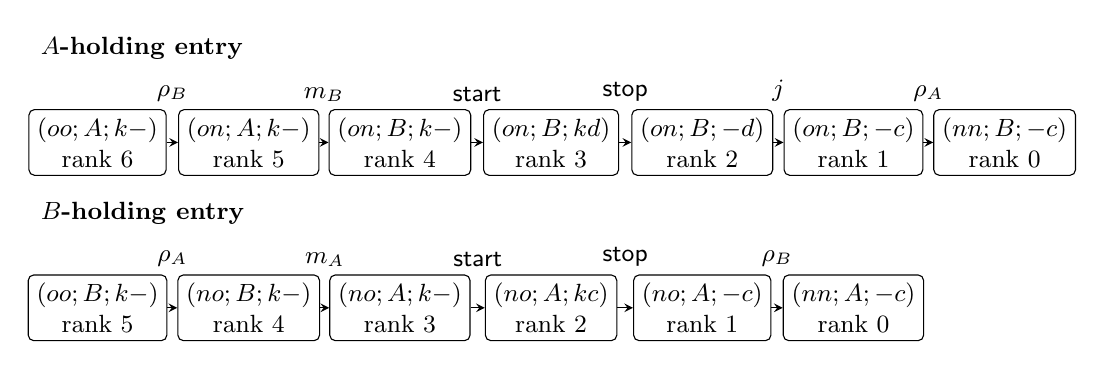
\begin{tikzpicture}[x=1.92cm,y=1cm,
  state/.style={draw,rounded corners=2pt,inner sep=3pt,font=\small,align=center},
  edge/.style={->,>=stealth},
  action/.style={font=\small,above,yshift=4mm}]
\node[anchor=west,font=\small\bfseries] at (-.44,1.2) {$A$-holding entry};
\node[state] (a0) at (0,0) {$(oo;A;k{-})$\\rank 6};
\node[state] (a1) at (1,0) {$(on;A;k{-})$\\rank 5};
\node[state] (a2) at (2,0) {$(on;B;k{-})$\\rank 4};
\node[state] (a3) at (3,0) {$(on;B;kd)$\\rank 3};
\node[state] (a4) at (4,0) {$(on;B;{-}d)$\\rank 2};
\node[state] (a5) at (5,0) {$(on;B;{-}c)$\\rank 1};
\node[state] (a6) at (6,0) {$(nn;B;{-}c)$\\rank 0};
\draw[edge] (a0)--node[action]{$\rho_B$}(a1);
\draw[edge] (a1)--node[action]{$m_B$}(a2);
\draw[edge] (a2)--node[action]{$\mathsf{start}$}(a3);
\draw[edge] (a3)--node[action]{$\mathsf{stop}$}(a4);
\draw[edge] (a4)--node[action]{$j$}(a5);
\draw[edge] (a5)--node[action]{$\rho_A$}(a6);
\node[anchor=west,font=\small\bfseries] at (-.44,-.9) {$B$-holding entry};
\node[state] (b0) at (0,-2.1) {$(oo;B;k{-})$\\rank 5};
\node[state] (b1) at (1,-2.1) {$(no;B;k{-})$\\rank 4};
\node[state] (b2) at (2,-2.1) {$(no;A;k{-})$\\rank 3};
\node[state] (b3) at (3,-2.1) {$(no;A;kc)$\\rank 2};
\node[state] (b4) at (4,-2.1) {$(no;A;{-}c)$\\rank 1};
\node[state] (b5) at (5,-2.1) {$(nn;A;{-}c)$\\rank 0};
\draw[edge] (b0)--node[action]{$\rho_A$}(b1);
\draw[edge] (b1)--node[action]{$m_A$}(b2);
\draw[edge] (b2)--node[action]{$\mathsf{start}$}(b3);
\draw[edge] (b3)--node[action]{$\mathsf{stop}$}(b4);
\draw[edge] (b4)--node[action]{$\rho_B$}(b5);
\end{tikzpicture}
\caption{One policy from both entries. States list versions of $A,B$, the workpiece holder, and old/new monitors; the holder also determines the interval monitor. A dash means inactive. Every edge decreases the remaining-step rank. The two rank-zero states match the respective fixed-controller targets.}
\label{fig:cell-paths}
\end{figure}


\subsection{Residual Soundness and the Cell Reference}\label{ta:residual_formal}
Residual soundness (RS) relates monitor memory to prior history. Let $\mathsf{SafePref}_r$ be requirement $r$'s prefix-closed language, and let $\mathsf H_r(\xi)$ contain all admissible activation histories consistent with observed component state $\xi$. A new requirement's history includes start once; its initialized monitor reads only later events. Residual-sound initialization means
\[
 \underbrace{\{w:\eta_r^*(\iota_r(\xi),w)\notin F_r\}}_{\text{continuations accepted by the initialized monitor}}
 \ \subseteq\
 \underbrace{\bigcap_{h\in\mathsf H_r(\xi)}\{w:hw\in\mathsf{SafePref}_r\}}_{\text{continuations safe after every admitted history}}
 \tag{RS}\label{eq:residual-soundness}
\]
for every $\xi\in\operatorname{dom}\iota_r$. Equality is exact; strict inclusion is conservative and may exclude feasible updates. An empty history set makes the right side universal. Synthesis checks initializer states and domains, but neither infers histories nor establishes their completeness.

For Cell's declared start-only reference, $\mathsf H_{r_{\rm inspect}}(\xi)=\{\mathsf{start}\}$. Initializing at $c$ is exact for that reference; initializing at $d$ when $B$ holds is conservative, forbidding departure until inspection. The complete inclusion proof is in Technical Appendix~\ref{ta:cell-residual}. This distinction exposes a separate obligation: an exact history residual need not encode the intended duty at activation.


A Boolean event-history variable, or \emph{fluent}, records setting/resetting labels. For an initially true fluent $p$, a history making $p$ false then true and the empty history end at the same value but differ under $\Box p$. 

\paragraph{Deriving RS in the cell.}\label{ta:cell-residual}
The declared pre-activation observation retains only $\mathsf{start}$, so $\mathsf H_{r_{\rm inspect}}(\xi)=\{\mathsf{start}\}$ for every admissible cell tuple. The reference monitor starts at $c$, unchanged by start; the right-hand side of RS is therefore its non-error continuation language from $c$. If $B$ is empty, initialization at $c$ gives equality. If $B$ holds, initialization at $d$ is conservative: before the first $j$ or $m_B$, $d$ additionally forbids $m_A$; either $j$ or $m_B$ brings the two initial states to the same state. Thus every word safe from $d$ is safe from $c$, while the single event $m_A$ witnesses strict inclusion. This is a proof for the declared observation scope, not recovery of pre-activation history.

Initializing at $c$ while $B$ holds satisfies equality but omits the intended pending-inspection duty encoded by $d$. Declared histories and intended obligations are therefore separate input choices.


\FloatBarrier









\FloatBarrier
\Needspace{6\baselineskip}
\section{Complete Benchmark Input Counts}\label{ta:benchmark_inputs}
Inputs have 1--5 components, 4--131 entries, 1--12 old/new requirements each and 3--26 commands, using PC2/R2's input log.
\begin{table}[!htbp]
\caption{The nine adapted inputs. Old/new requirements are shared across variants; interval counts are Base/R1/R2.}
\label{tab:input-structure}
\centering\small
\begin{tabular}{@{}lrrrrrr@{}}\toprule
Input & Comp. & Entries & Old/New & Interval B/R1/R2 & $T$ & $U$\\\midrule
GSM & \ContractGSMComponents{} & \FixedGSMEntries{} & \ContractGSMOld{}/\ContractGSMNew{} & \ContractGSMBase{}/\ContractGSMROne{}/\ContractGSMRTwo{} & \ContractGSMTransferPairs{} & \ContractGSMUpdates{}\\
Industry & \ContractIndustryComponents{} & \FixedIndustryEntries{} & \ContractIndustryOld{}/\ContractIndustryNew{} & \ContractIndustryBase{}/\ContractIndustryROne{}/\ContractIndustryRTwo{} & \ContractIndustryTransferPairs{} & \ContractIndustryUpdates{}\\
MetaSocket & \ContractMetaSocketComponents{} & \FixedMetaSocketEntries{} & \ContractMetaSocketOld{}/\ContractMetaSocketNew{} & \ContractMetaSocketBase{}/\ContractMetaSocketROne{}/\ContractMetaSocketRTwo{} & \ContractMetaSocketTransferPairs{} & \ContractMetaSocketUpdates{}\\
PowerPlant & \ContractPowerPlantComponents{} & \FixedPowerPlantEntries{} & \ContractPowerPlantOld{}/\ContractPowerPlantNew{} & \ContractPowerPlantBase{}/\ContractPowerPlantROne{}/\ContractPowerPlantRTwo{} & \ContractPowerPlantTransferPairs{} & \ContractPowerPlantUpdates{}\\
PC Arms=1 & \ContractPCOneComponents{} & \FixedPCOneEntries{} & \ContractPCOneOld{}/\ContractPCOneNew{} & \ContractPCOneBase{}/\ContractPCOneROne{}/\ContractPCOneRTwo{} & \ContractPCOneTransferPairs{} & \ContractPCOneUpdates{}\\
PC Arms=2 & \ContractPCTwoComponents{} & \FixedPCTwoEntries{} & \ContractPCTwoOld{}/\ContractPCTwoNew{} & \ContractPCTwoBase{}/\ContractPCTwoROne{}/\ContractPCTwoRTwo{} & \ContractPCTwoTransferPairs{} & \ContractPCTwoUpdates{}\\
Railcab & \ContractRailcabComponents{} & \FixedRailcabEntries{} & \ContractRailcabOld{}/\ContractRailcabNew{} & \ContractRailcabBase{}/\ContractRailcabROne{}/\ContractRailcabRTwo{} & \ContractRailcabTransferPairs{} & \ContractRailcabUpdates{}\\
Surveillance & \ContractSurveillanceComponents{} & \FixedSurveillanceEntries{} & \ContractSurveillanceOld{}/\ContractSurveillanceNew{} & \ContractSurveillanceBase{}/\ContractSurveillanceROne{}/\ContractSurveillanceRTwo{} & \ContractSurveillanceTransferPairs{} & \ContractSurveillanceUpdates{}\\
Workflow & \ContractWorkflowComponents{} & \FixedWorkflowEntries{} & \ContractWorkflowOld{}/\ContractWorkflowNew{} & \ContractWorkflowBase{}/\ContractWorkflowROne{}/\ContractWorkflowRTwo{} & \ContractWorkflowTransferPairs{} & \ContractWorkflowUpdates{}\\
\bottomrule\end{tabular}
\par\smallskip\footnotesize $T$ counts declared transfer pairs before fluent observers; $U$ counts transfer, stop and start commands. Entries agree across completed variants; PC Arms=2/R2 times out and its requirement counts come from its input log. Only Railcab has branching transfers. These nine inputs declare no explicit precedence; the separate cell witness requires $\mathsf{start}\prec\mathsf{stop}$; R2 uses interval monitors.
\end{table}


\paragraph{Requirement configurations.}
Each inherited input has three named requirement configurations: Base has no interval requirement; R1 protects selected actions during a requirement gap; R2 imposes selected ordering constraints. R1 blocks each designated action while its flag is true: any old-stop sets it, its designated new-start clears it. R2 requires selected boundaries before their transfers. In the GSM mobile-communication model, R1 blocks communication and decoding; R2 puts both decode-rule boundaries before transfer without ordering them. Event choices vary by model. PC2-Rolling, a production-cell calibration example, separately tests availability. The archived fork's traditional DUCS/GR backend (Legacy) also synthesizes subsequent control, a different objective.

\FloatBarrier

\FloatBarrier
\Needspace{19\baselineskip}
\section{All Completed Direct-Full Exploration Pairs}\label{ta:workload_rows}
The all-contract outcome summary is Table~\ref{tab:xeon-rq3} in the main paper. The table below reports every completed pair.

\begin{table}[!htbp]
\caption{Absolute exploration costs for all \FixedDirectFullPairs{} completed Direct-Full pairs. Figure~\ref{fig:rq3-outcomes} displays every fixed-budget contract for all four methods.}
\label{tab:workload-main}
\centering
% All 14 completed pairs; generated by build_rq3_workload14_W.py.
% Raw integers; solver seconds rounded to three significant digits.
\begingroup\small
\setlength{\tabcolsep}{3pt}
\renewcommand{\arraystretch}{1.04}
\begin{tabular}{@{}lrrr@{}}\toprule
Input / variant & States (L/DF) & Queries (L/DF) & Solver s (L/DF)\\\midrule
GSM / Base & 31 / 75 & 27 / 658 & 0.0224 / 0.0416\\
GSM / R1 & 34 / 115 & 44 / 706 & 0.0228 / 0.0450\\
GSM / R2 & 34 / 68 & 78 / 352 & 0.0201 / 0.0327\\
Industry / Base & 272 / 282,709 & 3,336 / 5,058,452 & 0.190 / 154\\
Industry / R2 & 7,717 / 51,096 & 52,919 / 725,391 & 1.15 / 28.0\\
MetaSocket / Base & 8 / 82 & 12 / 289 & 0.0149 / 0.0408\\
MetaSocket / R1 & 8 / 95 & 12 / 257 & 0.0136 / 0.0426\\
MetaSocket / R2 & 16 / 34 & 24 / 79 & 0.0152 / 0.0240\\
PowerPlant / Base & 73 / 8,168 & 165 / 47,618 & 0.0463 / 1.85\\
PowerPlant / R1 & 759 / 23,686 & 1,927 / 66,394 & 0.125 / 5.51\\
PowerPlant / R2 & 1,330 / 3,594 & 3,118 / 13,512 & 0.180 / 1.01\\
PC Arms=1 / Base & 83 / 407,019 & 840 / 3,842,690 & 0.0741 / 157\\
PC Arms=1 / R2 & 56,443 / 158,218 & 354,259 / 1,363,292 & 6.16 / 77.8\\
Railcab / R2 & 97,522 / 317,094 & 437,383 / 2,842,593 & 15.5 / 283\\
\bottomrule\end{tabular}\par
\smallskip\raggedright
L: Lazy; DF: Direct-Full. All 14 WIN/WIN pairs are shown. States and successor-oracle queries are exact first-trial counts. Solver seconds are medians of five valid runs, including internal checking and excluding JVM/frontend/endpoint time, rounded to three significant digits.
\par\endgroup

\end{table}

\FloatBarrier

\FloatBarrier
\Needspace{6\baselineskip}
\section{Default Exploration Order}\label{ta:exploration_order}
The RQ3 LTS configurations disable the preliminary guided search (both guided limits are zero). The complete algorithm queries every uncontrollable candidate first. If any such bucket is nonempty, it omits controllable queries by the UC-priority reduction. The underlying Post relation still contains any enabled ordinary controllable edges, which Direct-Full materializes. Otherwise lazy and update-first consume their sorted controllable cursor through the first nonempty bucket, deferring the rest; eager consumes every controllable candidate. A deferred candidate is never removed merely because it appears unpromising.

The default lazy/eager priority depends on the pending operations and endpoint projection, as follows. Entries in each row are tried from left to right; all listed types remain candidates if the game enables them.
\begin{center}\small
\begin{tabular}{@{}p{.40\linewidth}p{.56\linewidth}@{}}\toprule
Condition & Priority classes (first to last)\\\midrule
Some old stop pending & stop; transfer; ordinary; other update\\
No stop, some transfer pending & transfer; ordinary; other update\\
No stop or transfer, endpoint aligned & start; all other events\\
No stop or transfer, not aligned & events other than start; start\\
Update-first ablation & every update; every ordinary event\\\bottomrule
\end{tabular}
\end{center}
Within a class, the implementation prefers updates if update-first is configured or the endpoint projection is aligned, and ordinary events otherwise; remaining ties use type order start, transfer, stop, ordinary, then Java string order on the event label. Endpoint mismatch is the minimum over load signatures of the number of disagreeing component/new-monitor coordinates. An old coordinate agrees when its transfer contains the target; an inactive new monitor agrees when its defined activation map produces the target state.

$\mathsf{Open}$ is a LIFO stack. Initial roots and each newly discovered batch are sorted by increasing endpoint mismatch, then pending-set size, then canonical state order, and inserted in reverse so the least element is popped first. Existing stack entries keep their positions; this is not a global priority queue. Canonical ties compare component count, then each component's version and state, sorted active-monitor identifiers and states, and sorted pending labels; the problem's comparators define local state order. Already queued/expanded states are not inserted again. $\mathsf{Retry}$ is FIFO: append a state when it first has deferred candidates, remove from the head, skip winners/exhausted cursors, consume through the next nonempty bucket, and append again if candidates remain. Drain propagation after each expansion/resumption, and always serve $\mathsf{Open}$ before $\mathsf{Retry}$. These rules are implemented by \texttt{FineGrainedSuccessorOracle} and \texttt{OtfDucsSynthesizer}; the artifact retains their exact source. Eager changes bucket materialization and update-first changes candidate priority, providing the reported sensitivity checks without selecting an order after observing results.

\paragraph{Scope of the work bound.}
Let $d$ count discovered states, $c$ candidate queries (including empty results), and $o$ returned outcome incidences over those queries. Under the main paper's indexed-predicate, output-sensitive successor and constant-time bookkeeping assumptions, Algorithm~\ref{alg:otf} admits an implementation with $O(d+c+o)$ work and storage. This counts the finite explored portion, not the potentially exponential implicit game. It excludes endpoint preprocessing, representation-dependent predicate costs and the Java implementation's extra sorting/scanning.

\paragraph{Counters and charges.}
Intern each state once and queue its expansion once. A cursor advances monotonically through each state's finite candidates; thus each query and each cursor/Retry transition is charged to a candidate or state. For each queried nonempty bucket, retain an outcome counter and the maximum rank of already proved outcomes. An outcome pointing to a winner updates these immediately; otherwise store one reverse incidence at its target. When a state first enters the winning set, process each of its reverse incidences once. Hence all counter decrements and maximum updates total $O(o)$.

At a state with enabled uncontrollables, combine their returned outcomes into the required universal proving set; promotion is enabled only after every UC candidate has been queried. At a quiescent state, any nonempty control bucket whose counter reaches zero can certify promotion. Recording the first such bucket needs constant work per completed bucket. Nonempty flags prevent an empty bucket from certifying progress. A state is promoted at most once; its rank is one above its proving set's accumulated maximum, and the retained witness supports extraction.

Maintain Open, Retry and the promotion worklist by indexed membership and removable entries, so enqueue/dequeue/removal is constant time and exhaustion is detected without repeated global scans. Goal initialization and unsafe-state exclusion cost $O(d)$. The final policy traversal or losing-region extraction scans only stored states and incidences. Summing these charges proves the stated bound. The worklist computes the same monotone promotion fixed point as the abstract algorithm; this argument does not assert a linear running time for every implementation of its instruction to exhaust promotion.
\paragraph{Exploration containment and cost model.}
With indexed predicates, output-sensitive successors and constant-time bookkeeping, a counter implementation takes linear work in discovered states, queried candidates and returned outcomes (Technical Appendix~\ref{ta:exploration_order}). Endpoint preprocessing is excluded; Java additionally sorts transitions and scans entries (S2). Direct-Full constructs the whole reachable game with unsafe/goal terminals; Lazy may also reach it in the worst case.

Lazy discovers a subgraph of Direct-Full: induction over queries preserves shared entries, successors and terminal predicates. Neither expands unsafe states or goals; empty queries store no bucket.

\FloatBarrier

\FloatBarrier
\Needspace{6\baselineskip}
\section{Separate Extended-Budget Trials}\label{ta:extended_budget}
\paragraph{Extended-budget trials.}
Table~\ref{tab:extended-budget-main} separates single-trial populations on the same Xeon/JAR: \ExtFixedComparable{} comparable Direct-Full decisions match fixed-budget Lazy; \ExtFixedUncompared{} Travel $(4,8)$ WIN decisions resolve prior timeout.
Direct-Full timeouts, Surveillance/R1 heap exhaustion and Lazy PC2/R2 timeout persist at expanded heaps. The shared Travel $(6,1)$ timeout triggers the prespecified $(6,4)$ skip (records in S4).
\begin{table}[!htbp]
\caption{Separate enlarged-budget single trials (\ExtBudgetTimeCap{}~s cap). S4 retains every run, failure and skip.}
\label{tab:extended-budget-main}
\centering\small
\begin{tabular}{@{}llrrrrrr@{}}\toprule
Population & Heap (GiB) & Planned & WIN & LOSS & TO & OOM & Skip\\\midrule
Earlier (four methods) & \ExtBudgetInitialHeap{}/\ExtBudgetExpandedHeap{} & \ExtBudgetPlanned{} & \ExtBudgetWins{} & \ExtBudgetLosses{} & \ExtBudgetTimeout{} & \ExtBudgetOOM{} & \ExtBudgetSkipped{}\\
Eager & \VThreeExtSevenHeap{} & \VThreeExtSevenTrials{} & \VThreeExtSevenWin{} & \VThreeExtSevenLoss{} & \VThreeExtSevenTO{} & \VThreeExtSevenOOM{} & ---\\\bottomrule
\end{tabular}
\end{table}

% Generated ext7 intake; separate single trials, fixed-budget results unchanged.
\noindent On the same Xeon/JAR, Eager's \VThreeExtSevenHeap{}~GiB/\VThreeExtSevenCap{}~s single trials return \VThreeExtSevenWin{} WIN where Direct-Full remained unresolved at that heap, discovering about $(\VThreeExtSevenWinStatesMinTenMillions{}$--$\VThreeExtSevenWinStatesMaxTenMillions{})\times10^7$ states with UC pruning (\VThreeExtSevenWinRatioMinApprox{}--\VThreeExtSevenWinRatioMaxApprox{} times Lazy); Industry/R1 returns LOSS with \VThreeExtSevenIndustryROneStates{} states (\VThreeExtSevenIndustryROneRatio{} times).
All \VThreeExtSevenAgree{} decisions match fixed-budget Lazy; ratios concern decided pairs only.
The other \VThreeExtSevenUnresolved{} trials yield \VThreeExtSevenTO{} TO/\VThreeExtSevenOOM{} OOM at about \VThreeExtSevenFailureRSSMinWhole{}--\VThreeExtSevenFailureRSSMaxWhole{}~GiB peak RSS, a process-memory measure (S4).


\FloatBarrier

\FloatBarrier
\Needspace{6\baselineskip}
\section{NEW and UPD History-Scope Derivations}\label{ta:history_checks}
This appendix gathers the complete criteria and proofs for prior-history and entry-scoped requirements. S3 gives the measured frontend and its boundary conventions. These scopes are distinct from activation-scoped invariants in Appendix~\ref{ta:activation_scope}; none establishes platform conformance.

\subsection{Activation histories and residual meanings}
For prefix-closed requirement language $\mathsf{SafePref}_r$, let $\mathsf H_r(\xi)$ be the declared activation histories projected by $\mathsf{obs}_r$. NEW checks use safe prior histories (A); UPD checks begin their reference at entry (E). Whole-history meaning H is a separate diagnostic.

NEW activation histories include start once: initialization supplies the post-start residual and online monitoring consumes later events. Game admission initializes monitors without an update-game event; the FSP boundary interpretation below accounts for \texttt{hotSwapIn} once in the supplied UPD boundary state. Define $\mathcal C_r(\xi)=\bigcap_{h\in\mathsf H_r(\xi)}\{w:hw\in\mathsf{SafePref}_r\}$ and $\mathcal L_r(m)=\{w:\eta_r^*(m,w)\notin F_r\}$. Residual-sound initialization requires
  \[
    \mathcal L_r(\iota_r(\xi))\subseteq\mathcal C_r(\xi)
    \quad(\xi\in\operatorname{dom}\iota_r)
    \tag{RS}
  \]
with equality for an exact residual and strict inclusion for a conservative one. Distinct activation histories may require finite history bits in components and transfers. RS is supplied external interpretation evidence relative to the given requirement and observation meanings. For $r\in R^{\mathrm{upd}}$, $\operatorname{dom}\iota_r$ includes every reachable old component state.


\subsection{Safe prior histories for NEW requirements (A)}
A new requirement becomes effective at its own activation. Its supplied meaning retains the progress or obligations represented by the current fluent vector, while excluding prior violating histories from the reference intersection. With at most one occurrence of each update event, define
\[
 \mathsf H_r^{\rm safe}(\xi)=\{h\in\mathsf H_r(\xi):
    \eta_r^*(m_r^0,h)\notin F_r\},\qquad
 \mathcal C_r^{\rm safe}(\xi)=\bigcap_{h\in\mathsf H_r^{\rm safe}(\xi)}
    \mathcal L_r(\eta_r^*(m_r^0,h)).
\]
Then $\mathsf{RS}_A$ is $\mathcal L_r(\iota_r(\xi))\subseteq\mathcal C_r^{\rm safe}(\xi)$.
This is a choice of requirement meaning, not a proof that a past violating trace satisfied the original invariant. In particular, conditioning on safe histories does not validate application intent. If $\mathsf H_r^{\rm safe}(\xi)$ is empty, the intersection is the universal continuation language: inclusion is immediate, but equality generally fails. Exactness below is therefore explicitly restricted to nonempty safe-history domains.

\begin{lemma}[A: language-determined safe-prefix initialization]
\label{lem:rs-a}
Explore the freely reachable monitor/observer product over one-shot update histories, recording but not expanding ERROR pairs. Suppose all non-error monitor states reached at the same fluent vector have equal continuation languages. On the activation domain, let the actual non-error lookup $\sigma_r(v)$ have that common language. Then $\iota_r(\xi)=\sigma_r(f(\xi))$ satisfies $\mathsf{RS}_A$, with equality whenever $\mathsf H_r^{\rm safe}(\xi)\ne\varnothing$.
\end{lemma}
\begin{proof}
Every admissible safe history reaches a non-error product pair with observer vector $f(\xi)$. By language equivalence and lookup compatibility, its residual language equals $\mathcal L_r(\iota_r(\xi))$. A nonempty intersection of these equal languages is that language. For an empty history set, the universal intersection contains the initialized language, proving the stated inclusion.
\end{proof}
Language equivalence, rather than equality of state identifiers, is also the frontend's acceptance condition for multiple non-error states at a lookup vector. Our independent checker compares deterministic state pairs until an ERROR/non-error distinction or pair closure, and separately reconstructs the frontend's error-priority, equivalent-state/minimum-identifier rule. This checks the earlier saved monitor/observer exports against the source rule; those exports do not contain a materialized lookup table. A separate fresh frontend export directly checks all 138 tables (S4), while leaving general physical-state decoding and actual activation histories unverified. Appendix~\ref{ta:railcab-activation} separately analyzes two saved Railcab exports. The check establishes $\mathsf{RS}_A$ inclusion for all \RSAExactNew/\RSNewOccurrences{} NEW initializers without a nonemptiness premise. Equality additionally requires nonempty safe histories at the actual activation; their plant-level nonemptiness remains unverified.

\subsection{From update entry: UPD requirements (E)}
An update-interval requirement becomes effective at entry. Its reference monitor starts afresh with the actual entry fluent vector $v$, consumes \texttt{hotSwapIn} once, and observes the subsequent update interval. Let $\mathcal L_r^E(v)$ denote the resulting continuation language and $b_r$ the frontend's constant post-entry monitor state. For the entry vectors $V_r(\xi)$ compatible with $\xi$, define
\[
 \mathcal C_r^E(\xi)=\bigcap_{v\in V_r(\xi)}\mathcal L_r^E(v),
 \qquad \mathsf{RS}_E:\quad
 \mathcal L_r(b_r)\subseteq\mathcal C_r^E(\xi).
\]
The reference language must account for the effect of $v$ on monitor initialization; simply attaching an unused observer vector to the fixed compiled DFA does not establish that relation. Before and after the one entry occurrence, each other update label is permitted at most once in the sufficient-condition overapproximation. This overapproximation may admit update labels before entry that the actual game excludes.

\begin{lemma}[E: entry-value-independent boundary language]
\label{lem:rs-e}
Let $V_r$ overapproximate all reachable entry observer vectors under the one-shot event constraint. If $\mathcal L_r^E(v)=\mathcal L_r(b_r)$ for every $v\in V_r$, then the constant initializer satisfies $\mathsf{RS}_E$ exactly at every actual entry with nonempty $V_r(\xi)\subseteq V_r$.
\end{lemma}
\begin{proof}
Every actual entry vector belongs to $V_r$, so its reference post-entry language equals the boundary language by hypothesis. Thus the nonempty intersection over $V_r(\xi)$ consists of copies of $\mathcal L_r(b_r)$ and equals that language. Constant initialization uses $b_r$, giving equality in $\mathsf{RS}_E$.
\end{proof}
\begin{samepage}
\begin{lemma}[E$'$: update-stage fluents suffice]
\label{lem:rs-e-prime}
Suppose an UPD monitor references only declared fluents whose initiating and terminating labels are update commands: \texttt{stopOldSpec}, \texttt{startNewSpec}, \texttt{reconfigure} (including their indexed forms), or \texttt{hotSwapIn}. No such label occurs before actual entry. If the constant initializer is the non-error boundary state $b_r$ obtained from compiled state zero by consuming \texttt{hotSwapIn} once, then it satisfies $\mathsf{RS}_E$ with equality at every actual entry.
\end{lemma}
\begin{proof}
Before entry, no defining update label occurs, so all referenced fluents retain their declared initial values.
The fresh E monitor therefore starts at state zero and consumes \texttt{hotSwapIn} once, reaching $b_r$.
Every actual entry has reference language $\mathcal L_r(b_r)$, so the reference intersection equals that language.
\end{proof}
\end{samepage}
The E$'$ check reads the expanded initiating/terminating sets of each referenced fluent from the saved model exports, checks the constant initializer and its non-error boundary, and certifies \RSEExactUpd/\RSUpdOccurrences{} UPD occurrences. It uses the actual game's exclusion of pre-entry update commands; the older free-history diagnostic admits such commands and is retained unchanged. A name such as \texttt{stopPump} is an ordinary plant event, not an update command.

The historical E$'$ condition leaves \RSEUnverifiedUpd{} R1 occurrences unverified because they reference ordinary-action predicates. Attaching different observer vectors to a fixed DFA does not establish their reference languages. The additional source-specific check below proves their entry interpretation without changing those historical records.

\begin{lemma}[E: guarded-invariant entry initialization]
\label{lem:r1-entry}
For a fresh entry-scoped requirement $\Box(G\Rightarrow\neg A)$, suppose $G$ is initially false, changes only on actual update commands excluded from old-endpoint histories, and is unchanged by entry. Let $A$ be a disjunction of ordinary-event predicates, each reset by entry. If the saved DFA has the two-state invariant transitions described below and its constant initializer is the non-error false-guard state obtained by consuming entry once from its default initial state, then the initializer satisfies $\mathsf{RS}_E$ with equality at every actual entry.
\end{lemma}
\begin{proof}
No update command occurs before entry, so $G$ is false there. Every possible value of the action predicates satisfies the initial implication. Entry leaves $G$ false and resets all action predicates; the fresh pure invariant has no pending obligation from an earlier position. The resulting continuation language is thus identical for every entry valuation and equals that of the supplied boundary state. The compatible entry set is nonempty at an actual modeled entry, so intersecting these equal languages establishes exactness.
\end{proof}

The added checker reads the original source formulas, expands action aliases, and checks their correspondence to saved monitor/observer exports. For each R1 occurrence, it requires one default-false declared guard, nonempty disjoint initiating/terminating sets consisting only of actual update commands, and ordinary-event predicates reset by entry. It checks source/export equality of these sets, a constant non-error boundary initializer, and all DFA transitions against the two-state invariant: initiating commands set the guard, terminating commands clear it, a forbidden ordinary event when the guard holds enters ERROR, and other events stutter. ERROR absorbs all labels; absent local-alphabet edges become ERROR and labels outside that alphabet stutter, matching the adapter. All 46 monitors omit the entry label from their local alphabets, so consuming entry stutters at the false-guard state.

Inspection of namespace validation and endpoint construction, together with the saved successful input-validation results, establishes that old histories contain only ordinary events. The adapter computes the boundary value once and installs it directly at every old root; initialization does not consume entry a second time. Seven negative mutations test rejection of a wrong guard value, non-update guard event, guard-changing entry, missing declared edge/label, non-rejecting forbidden event and missing entry reset. The checker verifies all 46 occurrences across 4,722 state--label pairs and 854 possible action-predicate entry valuations. These are static validation counts, not extra synthesis trials or enumerated physical histories. S4 preserves the older free-history and E$'$ results, and the new CSV labels its distinct sufficient condition. The new proof uses the existing E meaning; it does not establish the history-inclusive H interpretation or application-level conformance.

\subsection{Whole-history obligations: a stronger diagnostic}\label{supp:history-diagnostic}
For this coverage audit, $\mathsf{obs}_r$ retains the events defining the referenced fluents, independently of the active component version. Run the requirement monitor from $m_r^0$ on the whole projected history before activation and its continuation. With absorbing error states this gives
\[
 \mathcal C_r(\xi)=\bigcap_{h\in\mathsf H_r(\xi)}
 \mathcal L_r\bigl(\eta_r^*(m_r^0,h)\bigr).
\]
H counts violations before activation. If an admitted history reaches ERROR, its continuation language is empty; a non-error initializer accepts the empty suffix and cannot satisfy RS at that activation. We retain the H check as a diagnostic and assert no benchmark RS guarantee under H. The A and E interpretations above have different scopes; none changes the compiled game or any saved synthesis decision.

\begin{lemma}[Fluent-determined exact initialization]
\label{lem:fluent-determined}
Let the freely reachable product of the deterministic requirement monitor (including absorbing errors) and all its referenced fluent observers start at their specified initial states. Suppose equal fluent vectors in that product imply equal monitor states. Let $\sigma_r(v)$ return that unique monitor state for each reachable vector $v$. For any activation state with $\mathsf H_r(\xi)\ne\varnothing$ whose histories are represented in this product and whose supplied initializer is $\iota_r(\xi)=\sigma_r(f(\xi))$, initialization is an exact residual for the history-inclusive interpretation.
\end{lemma}
\begin{proof}
Each projected activation history reaches a product pair $(\eta_r^*(m_r^0,h),f(\xi))$. Fluent determination makes its first coordinate equal to $\sigma_r(f(\xi))$, independently of $h$. Thus every language in the intersection defining $\mathcal C_r(\xi)$ is the same language $\mathcal L_r(\iota_r(\xi))$. Because the history family is nonempty, its intersection is that language, proving equality in RS. For an empty history family, the intersection is $\Sigma^*$ and this argument gives inclusion only, not equality in general.
\end{proof}

A single non-error state is insufficient for this lemma. For $[]p$ with $p$ initially true, let $a$ make $p$ false and $b$ restore it. The empty history and $ab$ have the same current fluent value but reach the safe and absorbing-error monitor states, respectively. A check that discards errors verifies only safe-prefix determination, a weaker condition that needs a separate safe-history premise. We use the full product, including errors. Failure of this plant-independent sufficient condition leaves RS unverified for the actual activation histories; it is not by itself a counterexample to the supplied plant's RS.


\FloatBarrier

\FloatBarrier
\Needspace{6\baselineskip}
\section{Proof of Conditional Trace Lifting}\label{ta:execution_proof}
\paragraph{Linking the phases.}
\label{def:link}
The linked model connects disjoint old/update/new phases by entry $z\mapsto\Init(z)$, policy edges $\SuccSet_\sigma$ and handover $q\mapsto\kappa(q)$. Here $\Init(z)$ is the admitted update state copied and initialized from old state $z$, $\SuccSet_\sigma$ gives the policy successors, and $\mathsf{CL}^v$ is the monitored closed loop of endpoint version $v$. Entry and handover add no game event. Let $\alpha$ be a phase-disjoint observation map.

\noindent\textbf{A1 (endpoints):} actual endpoint observations map to same-labeled edges of $\mathsf{CL}^v$ and preserve its component and monitor states.
\par\noindent\textbf{A2 (update observations and progress):} at a non-goal, filtering the complete environment event set disables every controllable event outside $\sigma(q)$ and disables no uncontrollable event; every remaining event/outcome maps into $\Post(q,a)$ and is reported with its successor identity. The resulting set is nonempty and a next event is eventually observed. This progress premise assumes no fairness among event choices.
\par\noindent\textbf{A3 (commands and observation):} each command starts at uncontrollable quiescence, finishes atomically and failure-free in finite time, and reports one modeled transfer or monitor-lifecycle transition with its successor identity. Internal $\tau$ steps, unobservable outcomes and divergence are outside the model.
\par\noindent\textbf{A4 (boundaries):} entry atomically observes the actual reachable old state $z$ and switches to $\Init(z)$; at a quiescent goal, ordinary controllables are disabled and handover installs its selected controller state and switches control. Each boundary is a finite, failure-free linearizable operation preserving the specified component and monitor states~\cite{HerlihyWing1990}.

For the history-based interpretation below, let $H_r^{\mathrm{exec}}(\xi)$ contain the actual activation histories at $\xi$, using the declared reference origin and event projection of $r$ (and consuming a new requirement's start exactly once). \emph{History completeness} is the explicit premise $H_r^{\mathrm{exec}}(\xi)\subseteq H_r(\xi)$ at every reached activation. It is not established by A1--A4 or by synthesis.

\begin{theorem}[Conditional trace lifting]
\label{thm:realization}
For a returned WIN certificate $(\sigma,\rank,\kappa)$ of an eligible contract, every execution satisfying A1--A4 maps through $\alpha$ to the linked model. From an observed entry $\alpha(x_0)=\Init(z)\in Q_0$, the update reaches quiescent handover within $\rank(\Init(z))$ observed game events and then hands control to the compatible endpoint. With history completeness and RS for a supplied initializer, its active interval satisfies the declared residual interpretation. Agreement with application intent remains an input obligation.
\end{theorem}


\begin{proof}
Fix an execution satisfying A1--A4 and a returned certificate $(\sigma,\rank,\kappa)$. We use the phase-disjoint observation map $\alpha$ from the theorem; the assumptions require it to preserve the specified component and monitor states, not merely event names. A1 maps the old prefix to same-labeled edges in the monitored old closed loop. At entry, A4 supplies one linearization point at which the actual reachable old state $z$ is observed and control changes to $\Init(z)\in Q_0$. Entry contributes the linked model's boundary edge and no game event. Thus the update observation starts in the certificate domain.

Suppose the current observation is a non-goal certificate state $q$. A2 filters controls according to $\sigma(q)$ while retaining every enabled UC event. Its next reported event and successor identity therefore give an edge $q\xrightarrow{a}q'$ in the complete policy successor relation. For a command, A3 additionally supplies the required UC quiescence, finite atomic completion and exact modeled successor. Ordinary reports satisfy A2 directly. The checked WIN certificate includes every such successor, so $q'$ remains safe and in its domain, with $\rank(q')<\rank(q)$. This establishes the update-prefix simulation and rank invariant by induction, for every outcome rather than a selected favorable one.

A2 makes a next event eventually observable at every non-goal; A3 rules out a nonterminating command between observations. Consequently the execution cannot stop or stall at a non-goal. An infinite sequence of update events would give an infinite strictly descending sequence of natural ranks, which is impossible. At most $\rank(\Init(z))$ game events therefore reach a goal. This is an event bound: the assumptions provide no uniform bound on the time between observations. They also impose no fairness on which enabled event or outcome occurs.

The goal predicate supplies UC quiescence and a compatible reachable new-endpoint state $\kappa(q)$. A4 disables ordinary controls, preserves the specified component and monitor states, and completes handover at a finite linearization point. Representing this operation by the linked boundary edge adds no game event. A1 then maps every new-phase observation to the selected monitored endpoint's same-labeled continuation. Thus the complete observed execution maps into the linked model. The argument assumes the two boundary implementations have the A4 properties; it does not prove their linearizability or atomicity from implementation code.

Finally, certificate safety preserves each supplied monitor while it is active. For each actual activation history, completeness places that history in the declared scope and RS includes the monitor's accepted continuations in the history's legal residual language. Applying this inclusion to every active interval gives the claimed requirement interpretation. The choice and intended meaning of those scopes remain input obligations. Unobservable transitions, divergence, failed commands and implementations violating A1--A4 are outside the theorem.
\end{proof}

\FloatBarrier

\section{Policy Requirement-Boundary Argument}\label{ta:policy_interpretation}
\paragraph{Opposing requirement boundaries.}
Policy's audits must overlap, but its old/new roles must not overlap. No precedence is supplied: the monitors force new-audit start before old-audit stop and old-role stop before new-role start. The saved policy interleaves these boundaries and its identity transfer; from the logged entry, service first clears the log. Grouping both starts makes the first global start overlap roles; grouping both stops makes the first global stop remove audit coverage. Both merged entries therefore lose, and the saved losing closure checks all alternatives. Ordinary events can be withheld, so this contract does not promise service continuity. The artifact gives its complete monitor/initializer/endpoint data.

\paragraph{A finite boundary witness.}
Policy(2) preserves audit coverage and excludes simultaneous old/new roles (Table~\ref{tab:policy-finite-c13}). Here $o,n$ mean old/new, $r$ running, $u,l$ unlogged/logged, $A,R$ audit/role, and $\ell_z,a_z$ mean log/access for version $z$.

\begin{table}[!htbp]
\centering\small
\caption{Complete finite-game input for Policy(2) under Section~\ref{sec:formalization}'s rules. All events are controllable. Unlisted monitor transitions self-loop, including at absorbing error $\mathsf{err}$; unlisted plant/controller edges are absent. Every monitor has alphabet $\Sigma$.}
\label{tab:policy-finite-c13}
\begin{tabular}{@{}p{.16\linewidth}p{.78\linewidth}@{}}\toprule
Part & Finite definition\\\midrule
Plant and transfer & Both versions have sole, initial state $r$, self-looping on $\SigmaN=\{\ell_o,\ell_n,\mathsf{service},a_o,a_n\}$. Transfer $\rho$ maps $r$ to $r$ and changes only its version tag.\\
Controllers & For $z\in\{o,n\}$, $C^z$ has alphabet $\SigmaN$, initial state $u$, edges $u\xrightarrow{\ell_z}l$, $l\xrightarrow{\mathsf{service}}u$, and $a_z$ loops at $u,l$. An unreachable third state has all $\SigmaN$ loops (the saved alphabet-padding state).\\
Endpoint monitors & Old: $A_o,R_o$; new: $A_n,R_n$. $A_z$ has states $u,l,\mathsf{err}$, initially $u$, and edges $u\xrightarrow{\ell_z}l$, $l\xrightarrow{\mathsf{service}}u$, $u\xrightarrow{\mathsf{service}}\mathsf{err}$. $R_z$ has states $\mathsf{ok},\mathsf{err}$, initially $\mathsf{ok}$, with $\mathsf{ok}\xrightarrow{a_{\bar z}}\mathsf{err}$ ($\bar z$ is the other version).\\
Interval monitor & States are $\{b\in\{0,1\}^4:(b_1\lor b_2)\land\neg(b_3\land b_4)\}\cup\{\mathsf{err}\}$, initially $1010$. Bits track active $(A_o,A_n,R_o,R_n)$. Commands $\mathsf{stop}_A,\mathsf{start}_A,\mathsf{stop}_R,\mathsf{start}_R$ set $b_1=0,b_2=1,b_3=0,b_4=1$, respectively; unsafe results enter $\mathsf{err}$. Ordinary events and $\rho$ preserve bits.\\
Commands and initializers & The four boundary commands and $\rho$ occur once each; precedence is empty. Stops deactivate old monitors; starts activate new ones. At either $(o,r)$ or $(n,r)$, initialize $A_n=u$, $R_n=\mathsf{ok}$; the interval initializer is defined only at $(o,r)$, returning $1010$. These domains are complete.\\
Entries and targets & For $x\in\{u,l\}$, entry $q_x$ admits $((o,r),C^o=x,A_o=x,R_o=\mathsf{ok})$, discards $C^o$, installs interval state $1010$, leaves new monitors inactive and marks all commands pending. Both $z_x=((n,r),C^n=x,A_n=x,R_n=\mathsf{ok})$ are targets. Goals require safety, no pending commands and a matching target; UC quiescence is automatic.\\
Boundary merge & One global start activates both new monitors; one global stop deactivates both old ones. Each monitor composes the two member transitions, audit then role. All other inputs remain fixed.\\\bottomrule
\end{tabular}
\end{table}

Lazy returns from $q_u$ $\mathsf{start}_A$, $\mathsf{stop}_A$, $\mathsf{stop}_R$, $\rho$, $\mathsf{start}_R$, traversing interval states $1010$, $1110$, $0110$, $0100$, $0100$, $0101$, then reaches $z_u$. From $q_l$, $\mathsf{service}$ first reaches $q_u$. Ranks five/six bound completion, not shortest length; this safe order is not unique. Audit overlap and a role-free interval are permitted.

Both merged entries lose: the first global start overlaps roles; the first global stop removes audit coverage. Either enters $\mathsf{err}$; ordinary events and transfer preserve these bits. Saved losing closure checks all alternatives, and merge validation confirms equal effects in both member orders.

These supplied games compare boundary granularity, without a DUCS expressiveness claim. Ordinary events can be withheld; service continuity is not required. Actual-history completeness, application adequacy and A1--A4 remain unestablished.

\FloatBarrier

\FloatBarrier
\section{Separate Evaluation Populations and All-Contract Grid}
\label{ta:additional_populations}
The following descriptions preserve the separate secondary populations reported in the main paper. They are not pooled with the fixed-budget comparisons.
Figure~\ref{fig:rq3-outcomes} displays all 108 fixed-budget outcomes. Figure~\ref{fig:rq3-direct-full-absolute} gives absolute costs for every completed Lazy/Direct-Full pair; main-paper Figure~\ref{fig:rq3-paired-absolute} compares Lazy with Eager under the same UC pruning.
% Generated from the fixed rq3-cells.csv and checked against its outcome macros.
\begin{figure}[!htbp]
\centering
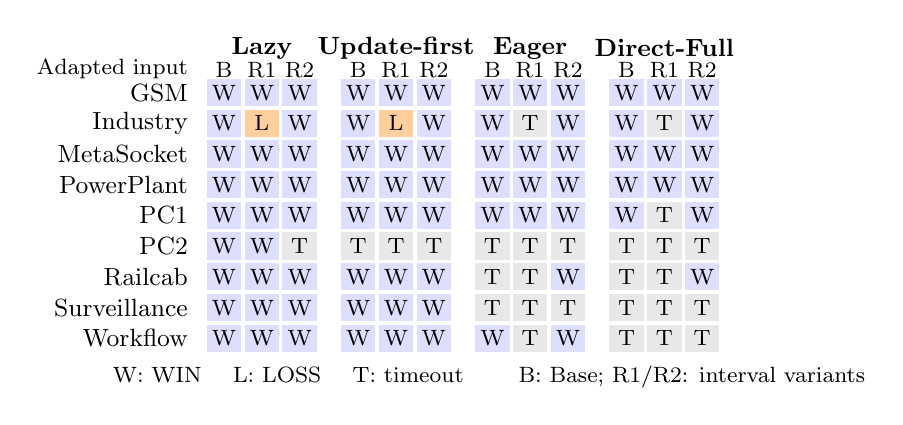
\begin{tikzpicture}[x=.48cm,y=.39cm,font=\small,
    cell/.style={draw=white,minimum width=4.5mm,minimum height=3.6mm,inner sep=0pt,font=\footnotesize},
    win/.style={cell,fill=blue!13,text=black},
    loss/.style={cell,fill=orange!38,text=black},
    timeout/.style={cell,fill=black!9,text=black}]
\node[anchor=east,font=\footnotesize] at (-.7,.75) {Adapted input};
\node[font=\small\bfseries] at (1.00,1.45) {Lazy};
\node[font=\footnotesize] at (0.00,.75) {B};
\node[font=\footnotesize] at (1.00,.75) {R1};
\node[font=\footnotesize] at (2.00,.75) {R2};
\node[win] at (0.00,0.00) {W};
\node[win] at (1.00,0.00) {W};
\node[win] at (2.00,0.00) {W};
\node[win] at (0.00,-1.00) {W};
\node[loss] at (1.00,-1.00) {L};
\node[win] at (2.00,-1.00) {W};
\node[win] at (0.00,-2.00) {W};
\node[win] at (1.00,-2.00) {W};
\node[win] at (2.00,-2.00) {W};
\node[win] at (0.00,-3.00) {W};
\node[win] at (1.00,-3.00) {W};
\node[win] at (2.00,-3.00) {W};
\node[win] at (0.00,-4.00) {W};
\node[win] at (1.00,-4.00) {W};
\node[win] at (2.00,-4.00) {W};
\node[win] at (0.00,-5.00) {W};
\node[win] at (1.00,-5.00) {W};
\node[timeout] at (2.00,-5.00) {T};
\node[win] at (0.00,-6.00) {W};
\node[win] at (1.00,-6.00) {W};
\node[win] at (2.00,-6.00) {W};
\node[win] at (0.00,-7.00) {W};
\node[win] at (1.00,-7.00) {W};
\node[win] at (2.00,-7.00) {W};
\node[win] at (0.00,-8.00) {W};
\node[win] at (1.00,-8.00) {W};
\node[win] at (2.00,-8.00) {W};
\node[font=\small\bfseries] at (4.55,1.45) {Update-first};
\node[font=\footnotesize] at (3.55,.75) {B};
\node[font=\footnotesize] at (4.55,.75) {R1};
\node[font=\footnotesize] at (5.55,.75) {R2};
\node[win] at (3.55,0.00) {W};
\node[win] at (4.55,0.00) {W};
\node[win] at (5.55,0.00) {W};
\node[win] at (3.55,-1.00) {W};
\node[loss] at (4.55,-1.00) {L};
\node[win] at (5.55,-1.00) {W};
\node[win] at (3.55,-2.00) {W};
\node[win] at (4.55,-2.00) {W};
\node[win] at (5.55,-2.00) {W};
\node[win] at (3.55,-3.00) {W};
\node[win] at (4.55,-3.00) {W};
\node[win] at (5.55,-3.00) {W};
\node[win] at (3.55,-4.00) {W};
\node[win] at (4.55,-4.00) {W};
\node[win] at (5.55,-4.00) {W};
\node[timeout] at (3.55,-5.00) {T};
\node[timeout] at (4.55,-5.00) {T};
\node[timeout] at (5.55,-5.00) {T};
\node[win] at (3.55,-6.00) {W};
\node[win] at (4.55,-6.00) {W};
\node[win] at (5.55,-6.00) {W};
\node[win] at (3.55,-7.00) {W};
\node[win] at (4.55,-7.00) {W};
\node[win] at (5.55,-7.00) {W};
\node[win] at (3.55,-8.00) {W};
\node[win] at (4.55,-8.00) {W};
\node[win] at (5.55,-8.00) {W};
\node[font=\small\bfseries] at (8.10,1.45) {Eager};
\node[font=\footnotesize] at (7.10,.75) {B};
\node[font=\footnotesize] at (8.10,.75) {R1};
\node[font=\footnotesize] at (9.10,.75) {R2};
\node[win] at (7.10,0.00) {W};
\node[win] at (8.10,0.00) {W};
\node[win] at (9.10,0.00) {W};
\node[win] at (7.10,-1.00) {W};
\node[timeout] at (8.10,-1.00) {T};
\node[win] at (9.10,-1.00) {W};
\node[win] at (7.10,-2.00) {W};
\node[win] at (8.10,-2.00) {W};
\node[win] at (9.10,-2.00) {W};
\node[win] at (7.10,-3.00) {W};
\node[win] at (8.10,-3.00) {W};
\node[win] at (9.10,-3.00) {W};
\node[win] at (7.10,-4.00) {W};
\node[win] at (8.10,-4.00) {W};
\node[win] at (9.10,-4.00) {W};
\node[timeout] at (7.10,-5.00) {T};
\node[timeout] at (8.10,-5.00) {T};
\node[timeout] at (9.10,-5.00) {T};
\node[timeout] at (7.10,-6.00) {T};
\node[timeout] at (8.10,-6.00) {T};
\node[win] at (9.10,-6.00) {W};
\node[timeout] at (7.10,-7.00) {T};
\node[timeout] at (8.10,-7.00) {T};
\node[timeout] at (9.10,-7.00) {T};
\node[win] at (7.10,-8.00) {W};
\node[timeout] at (8.10,-8.00) {T};
\node[win] at (9.10,-8.00) {W};
\node[font=\small\bfseries] at (11.65,1.45) {Direct-Full};
\node[font=\footnotesize] at (10.65,.75) {B};
\node[font=\footnotesize] at (11.65,.75) {R1};
\node[font=\footnotesize] at (12.65,.75) {R2};
\node[win] at (10.65,0.00) {W};
\node[win] at (11.65,0.00) {W};
\node[win] at (12.65,0.00) {W};
\node[win] at (10.65,-1.00) {W};
\node[timeout] at (11.65,-1.00) {T};
\node[win] at (12.65,-1.00) {W};
\node[win] at (10.65,-2.00) {W};
\node[win] at (11.65,-2.00) {W};
\node[win] at (12.65,-2.00) {W};
\node[win] at (10.65,-3.00) {W};
\node[win] at (11.65,-3.00) {W};
\node[win] at (12.65,-3.00) {W};
\node[win] at (10.65,-4.00) {W};
\node[timeout] at (11.65,-4.00) {T};
\node[win] at (12.65,-4.00) {W};
\node[timeout] at (10.65,-5.00) {T};
\node[timeout] at (11.65,-5.00) {T};
\node[timeout] at (12.65,-5.00) {T};
\node[timeout] at (10.65,-6.00) {T};
\node[timeout] at (11.65,-6.00) {T};
\node[win] at (12.65,-6.00) {W};
\node[timeout] at (10.65,-7.00) {T};
\node[timeout] at (11.65,-7.00) {T};
\node[timeout] at (12.65,-7.00) {T};
\node[timeout] at (10.65,-8.00) {T};
\node[timeout] at (11.65,-8.00) {T};
\node[timeout] at (12.65,-8.00) {T};
\node[anchor=east] at (-.7,0.00) {GSM};
\node[anchor=east] at (-.7,-1.00) {Industry};
\node[anchor=east] at (-.7,-2.00) {MetaSocket};
\node[anchor=east] at (-.7,-3.00) {PowerPlant};
\node[anchor=east] at (-.7,-4.00) {PC1};
\node[anchor=east] at (-.7,-5.00) {PC2};
\node[anchor=east] at (-.7,-6.00) {Railcab};
\node[anchor=east] at (-.7,-7.00) {Surveillance};
\node[anchor=east] at (-.7,-8.00) {Workflow};
\node[anchor=west,font=\footnotesize] at (-3.2,-9.25)
  {W: WIN \quad L: LOSS \quad T: timeout \qquad B: Base; R1/R2: interval variants};
\end{tikzpicture}
\caption{Every fixed-budget contract--method outcome. Each tile is one of the same
\ApplicationModels{} inputs $\times$ three requirement variants, under a
1,200~s cap and 64~GiB heap. WIN and LOSS are completed decisions; timeout leaves
feasibility unresolved. The methods change exploration, keeping entries,
successors and goals fixed. The comparison evaluates complete exploration procedures.
Workflow/R2's Direct-Full tile uses the recorded same-setting timeout after
interruption; both attempts are retained.}
\label{fig:rq3-outcomes}
\Description{A grid of all 27 contracts for each of four methods. Lazy has 25 WIN,
one LOSS at Industry R1 and one timeout at PC2 R2. Update-first has 23 WIN, one LOSS
and three timeouts. Eager has 17 WIN and ten timeouts. Direct-Full has 14 WIN and
13 timeouts. Every completed paired decision agrees.}
\end{figure}

\FloatBarrier
Base/R1/R2's 5/3/6 pairs give median state ratios 111.89/11.88/2.75 and solver ratios 40.02/3.12/9.14. The largest state savings are in Base, but different completed populations do not isolate interval requirements' effect.

\paragraph{Order sensitivity in R2.}
Eight R2 contracts complete all five repetitions with both Lazy and Update-first; PC2/R2 times out with both. Update-first discovers fewer states and has a lower solver median on Industry, PowerPlant, PC1, Railcab, Surveillance and Workflow; Lazy is lower on both measures for GSM and MetaSocket. For example, PC1/R2 has 56,443 versus 9,304 discovered states and 6.155 versus 1.166 seconds for Lazy versus Update-first. These saved results expose a substantial order dependence, but do not isolate a causal interaction between the order and interval monitors. The performance contribution concerns the full lazy procedure relative to construction alternatives, not a uniformly best exploration order.

\subsection{Complete records for the separate populations}
Supplement Sections~\ref{suppDoc-supp:vthree-ablations} and~\ref{suppDoc-supp:scaling} retain all Full+UC, restricted-transfer, controlled-family and Travel outcomes. Full+UC mixes builds, hosts and repetitions; its timing does not isolate UC pruning. For Legacy's subsequent-control reference, fixed-budget OOM/unmeasured cells are in Supplement Section~\ref{suppDoc-supp:fixed-budget}, source/fork discrepancies in Section~\ref{suppDoc-supp:legacy-reference}, and separate enlarged-heap trials in Section~\ref{suppDoc-supp:vthree-ext-six}. Other enlarged-budget failures and skips are in Appendix~\ref{ta:extended_budget} and Supplement Section~\ref{suppDoc-supp:extended-budget}; none enters fixed-budget medians.

The boundary fixture distinguishes forbidding an intervening event from merely merging same-type boundary labels (Supplement Section~\ref{suppDoc-supp:boundary-inputs}); Cell$_n$ and restricted-transfer controls follow in Section~\ref{suppDoc-supp:vthree-ablations}. The original finite-file results remain in Section~\ref{suppDoc-supp:independent-checks}; Section~\ref{suppDoc-supp:vthree-ablations} retains earlier failed inputs. Supplement Sections~\ref{suppDoc-supp:industry-diagnostic} and~\ref{suppDoc-supp:railcab-exports} give the complete Industry losing-region and Railcab policy diagnoses. Industry's global losing closure excludes every order; the validation-permitting variant changes the contract and supplies no timing data. The native DUCS WIN uses a different subsequent-control objective (main-paper Section~\ref{sec:railcab-policy}).

\subsection{Input adaptation details}
Nine inputs manually adapt eight DUCS sources; both ProductionCell sizes share a parent. Base/R1/R2 vary interval requirements, fixing components, transfers, endpoints and old/new goals (Technical Appendix~\ref{ta:benchmark_inputs}). Adaptations make PC tool results UC, revise Surveillance battery behavior/safety, order GSM/R2's decode boundaries before ENV transfer, shorten Railcab transfer paths while keeping both outcomes, and omit PowerPlant's explicit \texttt{ENV\_OLD}-to-\texttt{ENV\_NEW} transfer declaration while retaining \texttt{STARTED}-to-\texttt{STARTED}; the environment names alias those initial states. Recorded provenance does not establish whole-problem equivalence.

PC1/PC2 retain their DUCS parent's repeatable arrival cycle: UC $in_i$ enters an occupied arm; controllable $out_i$ and UC $reset_i$ permit its next arrival. With work and output withheld, pending tool results or reset/arrival chains finish in quiescent arm states. PC2-Rolling adds one UC calibration-completion step. This is finite drainage of pending physical events, not a total arrival budget or a safety proof. DUCS's production-cell study likewise distinguishes an empty-line condition from delaying newly arrived raw work~\cite[Sec.~6.1]{Nahabedian2020}. FG commands require no enabled UC event; a temporal gap between arrivals alone does not ensure this.

Travel couples an agency with $N$ amenities, $K$ UC choices and $0$--$K-1$ selection steps: size, branching and length covary. Adaptations change purchasing, admission, transfers and monitors without claimed trace equivalence. Supplement Section~\ref{suppDoc-supp:scaling} retains every setting and completed-pair comparison; $(N,K)=\FixedTravelAdditionalSettingsMath{}$ are the only settings extending OTF's fixed-budget decided range.

\paragraph{Independent-update construction.}
The complete $n+1$ versus $2^n$ construction and its proof occur once, in Supplement Section~\ref{suppDoc-supp:independent-family}. It assumes the measured pending-transfer-first query order and supplies no order-independent performance guarantee.

\subsection{Memory and returned policies}\label{ta:memory_policies}
Lazy's five-run median peak working sets span \FixedLazyRSSMin{}--\FixedLazyRSSMax{}~GiB (median \FixedLazyRSSMedian{}), including JVM/native overhead; Eager/Update-first sometimes use less. Its \FixedPolicies{} WIN certificates contain \FixedPolicyStatesMin{}--\FixedPolicyStatesMax{} update states (median \FixedPolicyStatesMedian{}) and maximum ranks \FixedRankMin{}--\FixedRankMax{} (median \FixedRankMedian{}). Ranks bound events, not downtime or optimal length. Counts match all five repeats; LOSS/TO has no winning policy.

The rank domain is recorded as \texttt{certificate\_states} in saved \path{rq3/stage1.csv}. S4's ``Output policy states'' instead uses \texttt{output\_controller\_states}: the linked old--update--new controller, with 15--1,260 states for Lazy. Linking includes reachable old and new closed-loop states and non-goal update states, identifying each update goal with its selected new state. These columns describe the same successful runs at different construction stages; neither counts explored game states.

\subsection{Lifetime gaps in two saved policies}\label{ta:saved-gaps}
The separate qualitative Railcab Base/R1 exports in S4 retain their full policy graphs. Define a gap on a completed path as the labels strictly after its last old-stop edge and strictly before its first new-start edge, excluding both boundaries. A normal label is outside the complete command set pending at entry. All 22 entries of each export have every old stop before the first new start on every possible policy path. There are 34 Base and 41 R1 completed paths when paths from different old entries are counted separately.
\begin{center}\small
\begin{tabular}{@{}lrrrr@{}}\toprule
Saved policy & States / edges & Entries & Gap labels & Ordinary gap labels\\\midrule
Railcab Base & 115 / 118 & 22 & 5--8 & 1--4\\
Railcab R1 & 44 / 46 & 22 & 3 & 0\\\bottomrule
\end{tabular}
\end{center}
The Base policy exploits a period without old or new requirements; R1 keeps its seven interval monitors active even when those requirements are inactive. The observed zero ordinary events in R1 describes this selected policy, not every winning policy. These counts quantify events, not elapsed time or suppressed alternatives.

The revised source's \path{scripts/analyze_saved_railcab_gap.py} traverses every saved outcome from every entry. It verifies entry coverage, strict rank decrease, one-shot command consumption, active-monitor membership, full certificate reachability and all terminal paths. Its inputs are the two \path{handoff-bundle.json} files under \path{results/supplement-checks/railcab_policy_demo/} and \path{results/supplement-checks/railcab_r1_policy_demo/}; it returns per-entry ranges and extremal path segments. Counting internal edges of the region with no active old/new monitor independently gives the same ranges for all 44 entries. The input bundles and this analysis script are included in the matching public snapshot.

This is a static analysis of the already saved qualitative exports, with no new synthesis or timing trial. Lazy's 125 successful fixed-budget repetitions instead retain summary-only controller output, certificate sizes and maximum ranks. Their unrecorded policy edges cannot establish corresponding gap ranges for all 25 WIN contracts. Neither these two exports nor their analysis reconstructs enabled but unselected events or an optimal completion rank.

\subsection{Separate Performance Populations}\label{ta:performance_scope_details}
The \FixedCensoredPairs{} capped Direct-Full attempts on Lazy-decided contracts give total-JVM lower bounds against Lazy medians, excluding PC2/R2 (both unresolved). These are single attempts, not solver ratios or medians; S4.5 retains all \ApplicationContracts{} absolute times/outcomes.

Full+UC matches Eager's state counts in \VThreeETwoEagerStateEqual{}/\VThreeETwoComparableEager{} cells; state-set equality is unchecked. OTF without pruning is unimplemented. Different builds, hosts and repetitions prevent single-factor timing claims. Technical Appendix~\ref{ta:additional_populations} also retains Legacy's subsequent-control reference and unresolved outcomes.

Controlled families agree on \FixedControlledWin{} WIN/\FixedControlledLossWord{} LOSS over \FixedControlledInputs{} inputs, without full factor isolation. Travel covaries agency/amenity size, branching and length: OTF gives \TravelOTFDecisions{} WIN/26 TO/2 OOM per method; Direct-Full gives \TravelFullDecisions{} WIN/28 TO/2 OOM. Both time out on $(6,1)$ at \ExtBudgetExpandedHeap{}~GiB/\ExtBudgetTimeCap{}~s. Technical Appendix~\ref{ta:additional_populations} retains extended TO/OOM/skips and the extended WIN versus fixed timeout at $(4,8)$; extended trials never enter medians.

\subsection{Finite contracts for the constructed families}\label{ta:constructed_contracts}
These definitions specify the inputs behind Table~\ref{tab:rq2-family-counts} and the Rolling grid. They describe finite models, not implementations of deployment platforms. Component versions have distinct tags even when their transition graphs coincide. Unlisted plant and endpoint-controller edges are absent; unlisted monitor labels stutter, and errors are absorbing. Ordinary events are controllable unless explicitly called UC. There is no explicit command precedence. OLD/NEW monitors are empty except in Rolling+Audit; the stated interval monitors apply until handover. The fixed endpoint graphs determine every reachable old entry and the listed loadable new targets. The main paper defines quiescence, command execution and the compared merges.

\paragraph{Rolling$(n,m)$ and block size $k$.}
For $2\leq n\leq6$, $1\leq m<n$, each old component has one ready state with a $serve_i$ loop. Its new version has booting and ready states, with UC $ready_i$ from booting to ready and $serve_i$ only at ready. A local transfer maps old ready to new booting. The interval monitor starts at $r=n$, decrements $r$ by the transferred block size, increments it on $ready_i$ (capped at $n$), and errors below $m$. Both fixed endpoints are all-ready tuples whose one-state controllers admit all $serve_i$ loops; these supply one entry and one target. Consecutive blocks of at most $k$, including the final remainder, are transferred atomically. The 15 $(n,m)$ pairs compare $k=1$ with $k=n$; the separate 70-cell grid varies $1\leq k\leq n$. Proposition~\ref{prop:rolling-threshold} proves the threshold for these inputs.

\paragraph{Canary$(n,m)$.}
The same 15 $(n,m)$ values use one old healthy state $H$ and new states $H,H_P,B_P,B$. Only $H$ serves. A transfer has two adversarial outcomes, $H_P$ and $B_P$; UC reports take $H_P$ to $H$ and $B_P$ to $B$. A controllable restart takes $B$ to $H$. The interval monitor is a bit vector initially zero: a broken report sets bit $i$, a restart clears it, and more than $n-m$ set bits cause error. Other labels stutter. This is a \emph{reported-broken} budget; pending physical states are not identified with already reported failures. The saved certificate also checks physical health separately. The all-healthy old/new tuples and one-state serve-only endpoint controllers give one entry and one target. Merging transfers synchronizes their commands and retains every Cartesian-product outcome. The healthy-outcomes-only and no-recovery variants restrict transfer images or remove restart, respectively; their unchanged both-WIN and both-LOSS results delimit the recovery mechanism.

\paragraph{Canary certificate scope.}
The existing separate check passed on every state of all 30 returned WIN certificates: the 15 parameter pairs under Lazy and Direct-Full. It counts replicas in $H$ or $H_P$ against the threshold $m$; $B_P$ and $B$ do not count. Thus it checks model-state health, while $H_P$ still cannot serve. It does not check continuous service, every explored state or runtime behavior. The other 30 saved checks concern LOSS mechanisms, not physical-health success. Fine and merged transfers share capacity reasoning with Rolling, but their reported-health contracts are different; no safety-preserving reduction to the Rolling game is claimed.

\paragraph{DB-Rolling$(3,m)$.}
Here $m\in\{2,3\}$. Each old component has primary $P$, secondary $S$, and election-pending $E$ states; the new version adds booting $B$. Serving loops exist at $P,S,E$. A controllable $stepdown_{i,j}$ synchronously changes $P_i$ to $S_i$ and $S_j$ to $E_j$; UC $elect_j$ changes $E_j$ to $P_j$. A transfer maps only $S$ to $B$, and UC $ready_i$ changes $B$ to $S$. The interval budget starts at three, decreases by the transferred block size, increases by one on readiness (capped at three), and errors below $m$; election does not consume this nonbooting budget. The old endpoint is $(P,S,S)$, the new target $(S,P,S)$, both with serve-only controllers; unreachable padding retains the remaining ordinary alphabet. Thus the contract specifies a change of primary. With $m=2$, a fine policy can change the primary and transfer secondary components successively. The merged command requires all-secondary states, which cannot be quiescent while an election remains pending. With $m=3$, even the first fine transfer violates the budget. These models do not assert uninterrupted write service.

\paragraph{Rolling+Audit.}
This is Rolling$(2,1)$ with controllable $log_{old}$ and $log_{new}$ loops in every local plant state. Each version's audit monitor has unlogged, logged and error states. Its own log sets logged; either serve changes logged to unlogged but errors from unlogged. The other log and all remaining labels stutter. The new initializer selects unlogged on all nine tagged physical tuples. The interval state is $(r,o,a)$, initially $(2,1,0)$: transfers/readiness change $r$ as above, old-stop clears $o$, and new-start sets $a$. Safety requires $r\geq1$ and $o\lor a$, enforcing overlap of the requirements. Each fixed all-ready endpoint controller alternates its own log with either serve; both its unlogged and logged states are entries/targets, and unreachable controller padding retains the remaining ordinary alphabet. These specify the memories, initializer and coverage obligation used in the comparison. Merging the two transfers loses; the single old-stop and new-start cannot be combined further, so merging requirement groups alone is only a renaming.

\paragraph{Threads$(n,B)$.}
For $2\leq n\leq6$ and queue capacity $B\in\{1,2\}$, each worker is idle or busy; component 1 additionally stores queue length $0\leq q\leq B$. UC arrival increments $q$ below capacity. At capacity, backpressure disables arrival whereas saturated arrival is a self-loop. Controllable $dispatch_i$ requires $q>0$ and worker $i$ idle, decrements $q$ and makes that worker busy; for $i>1$ it synchronizes with component 1. UC $finish_i$ returns a busy worker to idle. Old/new plant graphs coincide. Each local transfer is identity on idle states and preserves component 1's queue. There are no monitors. One-state endpoint controllers admit all ordinary labels; their reachable products from the empty, all-idle initial tuple give all old entries and all new targets. These two arrival modes yield 20 pairs. Under backpressure, disabling dispatch lets the finite queue fill and busy workers finish, permitting globally quiescent transfer. Saturated arrival can persist forever and prevents even fine transfer under the contract's quiescence rule. The negative control therefore distinguishes a genuine transfer opportunity from an implicit fairness assumption; it is not a reproduction of a multithreaded runtime.


\subsection{Granularity need not preserve feasibility}\label{ta:granularity-reverse}
The comparisons above do not assert that finer commands always retain every merged solution. The following analytical contract gives the reverse separation; it is not an additional measured instance or part of the 55-pair population.

Both components have one state per version and the shared ordinary alphabet $\{x,y,tick\}$, with $x,y$ UC and $tick$ controllable. Every version has a $tick$ self-loop. The only other loops are: $y$ in old component~1, $x$ in new component~1, $x$ in old component~2, and $y$ in new component~2. All other transitions are absent. Shared labels synchronize, so neither $x$ nor $y$ is enabled in the all-old or all-new product; $x$ loops in new/old and $y$ loops in old/new. Each local transfer maps its unique old state to its unique new state. There are no requirements, initializers or precedence edges. The one-state old and new controllers loop on all ordinary labels. Their closed loops each have one reachable state and a $tick$ loop, hence are safe and deadlock-free; these states supply the entry and target.

With separate transfers, either first transfer reaches a mixed state with an enabled UC self-loop. The remaining transfer is then permanently blocked by the quiescence rule; the environment can repeat the loop forever, so every fine policy loses. Merging both transfers into their single Cartesian-product command instead moves directly from the quiescent entry to the quiescent all-new target, with rank one. Thus fine LOSS/merged WIN is possible. Atomic merging can remove a harmful mixed state, whereas Cell and Rolling show that it can remove a necessary intermediate state. The reported obstructions establish when a specified merge loses, not a universal refinement order between granularities.


\clearpage
\section{Complete Native DUCS Construction for Cell}
\label{ta:ducs_cell_complete}\label{ta:ducs_interface}
Table~\ref{tab:ducs-interface} in the main paper compares the interfaces; the following construction makes that comparison concrete.

\begin{table}[!htbp]
\centering\small
\caption{Analytical Cell constructions: supplied and generated structures. No general translation, minimum-size, effort or performance result is claimed.}
\label{tab:main-generation}\label{tab:contract-interfaces-full}
\begin{tabular}{@{}p{.16\linewidth}p{.42\linewidth}p{.36\linewidth}@{}}\toprule
Interface & Supplied Cell structure & Generated or selected structure\\\midrule
DUCS~\cite[Defs.~4.1--4.3, 5.1]{Nahabedian2020} & Holder-refined old controller; environment transfer $R$; eight version/holder and three endpoint states in $E'$; guarded transfers, fluent goals $G,G',T$ and eventual handover $h$ & Protocol/interrupt composition, update environment/goal, update-and-subsequent controller with map $H$; legal, deadlock-free completion from all old-controller states\\
GR(1) update~\cite[Def.~3.1, Secs.~4--4.1]{Amram2022GR1DynamicUpdate} & Phase-extended specifications with version/lifetime variables, transfer guards, $p'=[h=B]$ at start, old inspection ban released at stop, switching condition and endpoint edges & New controller $C_2$, bridge and switching bookkeeping; bounded switch from winning states, then $C_2$ unchanged\\
FG-DUCS & Local components, $g_A=g_B=\{(e,e)\}$, typed monitors, initializers, start-before-stop, endpoint controllers and $Z_{\mathrm{load}}=\{z_A,z_B\}$ & Mixed-state and boundary transitions, target tests; policy, rank and handover map preserving the supplied continuation\\\bottomrule
\end{tabular}
\par\smallskip{\footnotesize The eight stages record versions and holder, excluding protocol and monitors. FG-DUCS's new-monitor initializer also covers all eight tuples. All three interfaces require justified input meanings.}
\end{table}


We construct a correct Cell update using native DUCS environments, relation $R$, transition requirement $T$ and boundary protocol $O$~\cite[Defs.~4.1--4.3 and 5.1]{Nahabedian2020}.

DUCS's \texttt{hotSwap} event requests the update and interrupts old control. Its \texttt{reconfigure} milestone switches environments; our extra $h$ connects mixed stages to a fixed endpoint.

\paragraph{Environments and entry.}
Refine the old controller to its reachable closed loop $c_A\xrightarrow{m_B}c_B\xrightarrow{m_A}c_A$, preserving ordinary traces and recording the holder. The old environment has these same moves. Let $E'$ contain eight stages $(v_A,v_B,L)\in\{o,n\}^2\times\{A,B\}$ and three post-handover states. In a stage, $m_B$ moves $A$ to $B$, $m_A$ moves $B$ to $A$, and $j$ self-loops only if $v_B=n,L=B$. Transfer $\rho_i$ changes $v_i=o$ to $n$ only while station $i$ is empty. A controllable $h$ maps $(n,n,L)$ to $z_L$. Post-handover edges copy the fixed new closed loop:
\[
z_A\xrightarrow{m_B}y_B\xrightarrow{j}z_B,
\qquad z_B\xrightarrow{j}z_B,
\qquad z_B\xrightarrow{m_A}z_A.
\]
Here $y_B$ is inspection-pending; $z_A,z_B$ are clear targets. The standalone initial state is $z_A$, but interrupt entry uses $R:L\mapsto(o,o,L)$. The 11-state count excludes protocol and monitors and is not a minimality result.

\paragraph{Requirements and memory.}
Write $s=\mathsf{startNewSpec}$ and $t=\mathsf{stopOldSpec}$. Protocol $O$ accepts these physical stutters. Let $\dot a$ record last event $a$, resetting on every other label. Fluents $B=\langle m_B,m_A,\mathsf{false}\rangle$ and $P=\langle m_B,j,\mathsf{false}\rangle$ retain holder and uninspected-arrival history. Take $G=\neg\dot j$ and $G'=\neg(P\land\dot m_A)$ under native old-until-stop and new-after-start scopes.

For each event $a$, let $S_a$ be its initially false, never-reset occurrence flag. Take $T$ to be the conjunction
\[
\begin{aligned}
&\Box(\dot s\Rightarrow S_{\mathsf{reconfigure}}),
&&\Box(\dot t\Rightarrow S_s),\\
&\Box(\dot h\Rightarrow S_{\rho_A}\land S_{\rho_B}\land S_s\land S_t\land\neg(B\land P)),
&&\Box(\dot{\mathsf{reconfigure}}\Rightarrow\Diamond\dot h).
\end{aligned}
\]
Interrupts, $O$, version guards and the post-handover region ensure at most one occurrence of each update event. This analytical $T$ includes eventual $h$, beyond the published safety-$T$ implementation~\cite[Sec.~5.3]{Nahabedian2020}; no solver experiment is claimed.
Native DUCS still requires eventual $\mathsf{stopOldSpec}$, $\mathsf{reconfigure}$ and $\mathsf{startNewSpec}$, including in its safety-$T$ implementation. Here $\mathsf{reconfigure}$ enters the mixed stages; $h$ is an additional fixed-target connection, so those three milestones do not by themselves require $h$. We do not rule out another encoding within safety-$T$.

\begin{proposition}[Cell witness preservation]
\label{prop:cell-ducs-complete}
This staged native DUCS instance admits a correct update from both reachable old entries. On the segment from $\mathsf{hotSwap}$ through $h$, erasing these two events and $\mathsf{reconfigure}$ and renaming $s,t$ to Cell's boundaries gives the displayed FG policy paths. After $h$, its ordinary traces equal those of the supplied new closed loop rooted at the selected target.
\end{proposition}
\begin{proof}
Use DUCS's assembled environment, including $O$, its old-event renaming/fluent extension, and controller extraction~\cite[Sec.~5, Theorem~5.1]{Nahabedian2020}. Preserve old behavior before $\mathsf{hotSwap}$. Map $H(c_L)$ to the corresponding pre-reconfiguration controller state; then choose $\mathsf{reconfigure}$, the six-/five-event path of Figure~\ref{fig:cell-story}, $h$, and every fixed-endpoint edge thereafter. All choices are enabled in the assembled environment; no ordinary UC event remains after initiation, ensuring legality and deadlock freedom.

Old $j$ is disabled until $t$. On safe active prefixes the correspondence is: the FG monitor is pending iff $B\land P$. At $s$, a $B$ holder has an earlier $m_B$ and no $j$, so both are pending. At an $A$ holder, $B$ is false and FG is clear, although $P$ may remain true from an earlier visit to $B$. This is equivalence of permitted continuations on the plant, not equality between $P$ and the monitor state: $m_A$ and $j$ are disabled at $A$, and the next $m_B$ makes both representations pending. Thereafter $j$ clears $P$ and the monitor. An enabled $m_A$ comes from $B$; it leaves $P$ unchanged while setting $\dot m_A$, so it violates $G'$ exactly when FG was pending. Otherwise it leaves $B\land P$ and FG clear. Transfers and boundaries preserve the correspondence. Thus every ordinary extension has the same safety outcome in both representations. The finite paths satisfy the boundary order and reach all-new, clear targets, fulfilling $T$ and the native update milestones. After $h$, the synchronized environment/controller copies retain every fixed-endpoint edge. Their reachable product is diagonal, giving the claimed ordinary-trace equality.
\end{proof}

The native encoding explicitly supplies stages, guards, holder refinement, history fluents, target gate and post-handover graph. FG-DUCS generates the update-game counterparts from local transfers, lifecycle rules, initializers and fixed targets, returning rank and handover certificates. This deterministic, fully controllable example establishes one-direction witness preservation, not a general translation, solution-set equivalence, measured effort saving or performance advantage.

\paragraph{Comparing the supplied structure.}
We count the same semantic objects in the three displayed Cell constructions (Appendices~\ref{ta:cell}, \ref{ta:ducs_cell_complete}, \ref{ta:gr1-cell}). Their shared reference endpoint graphs have two states/two edges (old) and three states/four edges (new), with two load targets. Table~\ref{tab:cell-input-responsibilities} tracks how the same Cell objects are encoded. Its rows are not additive input-size or effort measures.

\begin{table}[!htbp]
\centering\small\setlength{\tabcolsep}{4pt}
\caption{The same Cell objects through three explicit input constructions. Counts describe these constructions, not minimum encodings.}
\label{tab:cell-input-responsibilities}\label{tab:contract-responsibility}\label{tab:ducs-interface}
\begin{tabular}{@{}>{\raggedright\arraybackslash}p{.17\linewidth}>{\raggedright\arraybackslash}p{.26\linewidth}>{\raggedright\arraybackslash}p{.26\linewidth}>{\raggedright\arraybackslash}p{.25\linewidth}@{}}\toprule
Common object & FG-DUCS & Chosen DUCS input & Chosen GR(1) input\\\midrule
8 version/holder configurations & Generated one-workpiece physical projection of the local component product. & 8 mixed stages supplied in $E'$. & 8 valuations of supplied coordinates $h,v_A,v_B$.\\[3pt]
2 empty-station transfers & Two supplied singleton relations $g_A,g_B$; guarded commands generated. & Two transfer labels with version/empty-station guards in $E'$. & Two guarded-assignment rows in $R_B$.\\[3pt]
2 requirement boundaries and 1 order & OLD/NEW types and supplied $s\prec t$ generate boundary guards and active lifetimes. & Native $s,t$, with their ordering clause in $T$. & Supplied bits $s,t$ and the stop row's ordering guard.\\[3pt]
Inspection duty at start & Supplied holder-dependent initializer installs pending iff $B$ holds. & Supplied history fluents $B,P$ and $G'$ retain the corresponding duty. & Supplied start assignment $p'=[h=B]$.\\\bottomrule
\end{tabular}
\par\smallskip{\footnotesize DUCS generates its standard protocol $O$ and interrupt composition; GR(1) generates its bridge and switch bookkeeping. These are not extra modeler inputs.}
\end{table}

The modeler still supplies FG-DUCS with three monitors: eight states and eight explicitly listed nondefault edges in Table~\ref{tab:cell-finite-main}, before adding default self-loops and absorbing-error edges. The other constructions encode the one-workpiece invariant directly in the holder coordinate. Thus local generation does not remove all modeling obligations or show fewer supplied objects. The DUCS target gate and post-handover graph retain all four endpoint edges; the GR(1) post relation permits them, but its synthesized $C_2$ may retain fewer. FG-DUCS instead takes the fixed controllers and targets as inputs and generates their matching tests. The demonstrated difference is the generation of mixed stages and lifetime operations from the local contract, not a measured effort or size advantage.


\FloatBarrier
\section{Saved PC2 Activation Histories and Their Boundary}
\label{ta:pc2_history_boundary}
The supplied old controller and pre-synthesized new controller are fixed. Baseline PC2's old requirements and \ContractPCTwoNew{} new requirements remain; added new-endpoint calibration availability yields \PCTwoTraceNewStarts{} new starts, separate from the interval duty. Transfers map old destinations to calibration counterparts, retaining ordinary observer memory. Work, calibration requests and updates are controllable; arrivals, tool outcomes, resets and calibration completion are UC. Entry inherits old memory and initializes the interval monitor; new-start looks up the current ordinary observer tuple. No precedence is supplied. Targets match components and new-monitor memory at reachable new-endpoint states.

Interval $R_{CAL\_READY}$ observes transfers as calibration entry; endpoint availability observes ordinary requests. Completion restores both. Handover matches component, observer and new-monitor memory; real-history and runtime obligations remain unvalidated.


\paragraph{Generation responsibilities beyond Cell.}\label{ta:pc2-generation}
PC2 separates an application obligation from its generated update protocol. The designer supplies the two old/new arm models, their local transfer maps, twelve old and thirteen new requirements, the interval duty and fixed endpoints. For interval availability, each readiness bit starts true, becomes false on its arm's transfer or calibration request, and becomes true on completion; their disjunction must hold. This obligation is supplied, not inferred from the plant.

From these inputs, FG-DUCS constructs the twenty-five independent requirement boundaries and two local transfers, their active-monitor updates, mixed-version successors, UC-quiescence guards and target tests. The frontend prepares current-observer lookup maps and physical closure; the lazy solver generates the update product on demand. The saved result covers 126 entries with 381 policy states, 522 edges and maximum rank 37. Thus neither the sequence nor those policy states are part of the input. These counts describe one saved result, not a bound on the full mixed product.

For the published DUCS interface, a representation of these independently changing arms and requirement memories would place their staged behavior and admissibility in the supplied $E'$ and transition requirements. DUCS itself still generates its global update protocol; that work is not assigned to the designer~\cite[Secs.~4.2, 5]{Nahabedian2020}. A GR(1) representation would supply corresponding version, local-state, active-memory and observer variables with transition constraints; its existing construction generates switching bookkeeping and the bridge~\cite[Def.~3.1, Sec.~4]{Amram2022GR1DynamicUpdate}. Unlike the deterministic Cell construction, PC2 has UC outcomes, so this responsibility comparison does not establish an equivalent GR(1) game or a general translation. It identifies which local operations FG-DUCS generates directly, without measuring modeling effort, minimum encoding size or external-solver performance.


\begin{table}[!htbp]
\caption{One saved \PCTwoTraceEvents{}-event PC2-Rolling path. O/N: old/new; ARM: unprocessed workpiece; CAL: its calibration counterpart. Ordinary observers stay zero.}
\label{tab:pc2-saved-path}
\centering\small
\begin{tabular}{@{}p{.41\linewidth}llrr@{}}\toprule
Reached after & Arm 1 & Arm 2 & Available & Rank\\\midrule
Update entry & O/initial & O/initial & 2 & 31\\
Two arrivals, twelve old stops & O/ARM & O/ARM & 2 & 17\\
Transfer arm 1 & N/CAL & O/ARM & 1 & 16\\
Calibration completion 1 & N/ARM & O/ARM & 2 & 15\\
Transfer arm 2 & N/ARM & N/CAL & 1 & 14\\
Calibration completion 2 & N/ARM & N/ARM & 2 & 13\\
Thirteen new starts: handover & N/ARM & N/ARM & 2 & 0\\\bottomrule
\end{tabular}
\par\smallskip{\footnotesize At handover, all 13 new monitors are 0 and no command remains; the matched endpoint has both arms operational. Certificate identifiers are in Technical Appendix~\ref{ta:pc2_history_boundary}. This path supplies no timing and does not replace all-entry/all-outcome checking.}
\end{table}


This analysis traverses existing PC2-Rolling exports; it runs no solver and adds no timing trial. The selected requirement is $\Box(out_1\Rightarrow Drilled_1\land Cleaned_1\land Painted_1)$. The three fluents start false, successful tool events set them, and $reset_1$ clears them. An $out_1$ with any false fluent violates the requirement. Other update commands stutter for these fluents.

The saved old closed loop contains 126 reachable states and 348 edges; the policy contains 381 states and 522 edges. Its maximum state and entry rank is 37; all 522 edges decrease rank, and the longest entry-to-goal path has 37 events. The stored certificate therefore covers all 126 entries; the rank-31 path below is one representative. Matching component states, old-monitor memory and ordinary observers identifies each policy entry with one old state. Every maximal policy run crosses the single selected start edge $q_{13}\to q_{12}$, which installs monitor state 0 at two NEW/ARM components with all 24 ordinary observers zero. Ranks strictly decrease; removing that start edge makes the unique goal unreachable from every entry.
The path in Table~\ref{tab:pc2-saved-path} starts at $q_{126}$ and ends at $q_7$, whose handover target is \texttt{new-00000009}. All 13 new monitors are 0 there and no command remains. Its prefix to $q_{12}$ has two arrivals, twelve stops, four transfer/completion events and eight starts, with no $out_1$ or successful tool result.

For each entry, find an old prefix from the declared old initial state and a policy prefix ending at this start. Keep an edge only if the source fluent values and its label do not violate the selected new requirement. Forward reachability in the old graph and reverse reachability from the start in the policy graph yield the table. Separate per-entry breadth-first traversals construct positive witnesses or record failure of each portion; set-based fixed points reproduce the same partition.

\begin{center}\small
\begin{tabular}{@{}llr@{}}\toprule
Safe old prefix exists & Safe policy prefix exists & Entry count\\\midrule
Yes & Yes & 39\\
No & Yes & 21\\
Yes & No & 66\\\bottomrule
\end{tabular}
\end{center}
All 126 entries reach the start through some unrestricted saved-model history. The 39 positive rows establish existential nonemptiness at this one reached tuple, not safety of all histories. An old cycle
\[
in_1;drill_1;drillOk_1;polish_1;polishOk_1;clean_1;cleanOk_1;out_1;reset_1
\]
returns to the identical old initial tuple. It violates the new requirement at $out_1$ because $Painted_1$ is false. Prepending this cycle to any entry's history preserves its final activation tuple while retaining a past violation. The new monitor is absent in every old state and all 375 policy ancestors of its start, so none of these negative histories refutes its active-lifetime safety. They show why activation-safe and history-inclusive scopes cannot be conflated.

Replay of source-declared plant moves and all 24 observer updates agrees with all 348 old and 522 policy edges. This establishes consistency of these saved histories, not independent frontend correctness or completeness of exported outcomes. The artifact retains all 126 rows, positive paths, negative reasons and 18 boundary edges separating the safe reachability sets. Only one reached tuple of one requirement is covered; the reported 38,288 initializer guard tuples, the other 12 PC2 new requirements and the 138-occurrence population are not checked for nonemptiness by this analysis.

\paragraph{Direct ACT argument after the selected start.}
ACT begins the invariant with the actual observer values at activation. For the selected requirement these values are all zero. The saved policy graph's complete suffix is:
\begin{center}\small
\begin{tabular}{@{}lll@{}}\toprule
Source (rank) & New requirement started & Target (rank)\\\midrule
$q_{12}$ (5) & \texttt{OUT\_IF\_FINISHED\_2} & $q_{11}$ (4)\\
$q_{11}$ (4) & \texttt{TOOL\_ORDER\_1} & $q_{10}$ (3)\\
$q_{10}$ (3) & \texttt{TOOL\_ORDER\_2} & $q_9$ (2)\\
$q_9$ (2) & \texttt{PAINT\_ONCE\_1} & $q_8$ (1)\\
$q_8$ (1) & \texttt{PAINT\_ONCE\_2} & $q_7$ (0)\\\bottomrule
\end{tabular}
\end{center}
All six states have two NEW/ARM components, 24 zero observers and selected-monitor state 0. No ordinary event, transfer or uncontrollable edge occurs in this suffix. The unique goal matches \texttt{new-00000009}. Consequently the source invariant holds at activation and on every remaining update step; matching the verified new endpoint supplies its post-handover guarantee.

The saved graph is closed over 381 entry-reachable states; all 522 edges decrease a natural rank, and no non-goal deadlocks. Removing the unique selected start leaves 375 reachable states and no goal from any of the 126 entries. Thus every maximal saved-policy run crosses the start and follows this suffix. The static checker \path{check_saved_suffix.py} reproduces these facts from the existing certificate without invoking synthesis. Completeness of modeled outcomes relies on the stored certificate checker; frontend/compiler correctness and real execution are not independently proved here. The argument concerns one requirement and one reached tuple, not all 138 NEW occurrences. The A/H diagnostics above remain unchanged.

\subsection{All New Requirements of the Saved PC2 Policy}\label{ta:pc2_all_act}
The previous history analysis fixes one requirement to distinguish A from H. A separate inspection of the same saved policy establishes the active-lifetime obligation for all thirteen new requirements. It introduces no solver run, input change or timing trial.

The only new-start edges are the chain $q_{20}\to q_{19}\to\cdots\to q_7$, in this order: stamping avoidance for arms 1 and 2; calibration availability; clean-once for arms 1 and 2; drill-once for arms 1 and 2; output-if-finished for arms 1 and 2; new tool order for arms 1 and 2; and paint-once for arms 1 and 2. The selected start above is the eighth edge. Every state in this chain has two NEW/ARM components, all 24 ordinary observers zero and rank $q-7$ at $q$. Each newly installed monitor is 0 and stays 0. There is no ordinary event, transfer or UC edge after the first new-start.

\begin{proposition}[All PC2 active obligations]\label{prop:pc2-all-act}
Every maximal run of the saved PC2-Rolling policy from any of its 126 entries activates all thirteen new requirements and satisfies each source invariant from its own activation through handover. The matching verified new endpoint preserves these obligations afterward.
\end{proposition}
\begin{proof}
The saved domain is entry-reachable and closed, every edge strictly decreases a natural rank, and no non-goal deadlocks. Hence every maximal run reaches the unique goal $q_7$. Every $q_j$, $7\le j\le19$, has only its preceding chain edge as an incoming policy edge, and no entry lies on the chain. Thus every run traverses all thirteen starts.

For each arm, the source invariants forbid stamping; forbid cleaning, drilling or painting an already completed workpiece; require all three completed-tool fluents at output; and constrain tool-pending fluents by the new tool order. At activation all completed-tool and pending fluents are false, and no ordinary action occurs on a start label. Each invariant therefore holds. The calibration invariant is $\Box(\neg Calibrating_1\lor\neg Calibrating_2)$. Its source fluents start false and are set only by ordinary calibration requests. The old plant has no such request, so every old entry retains false values; none occurs in this policy either, while completion clears them. They too are false on the start chain. Start commands preserve these fluents and produce no ordinary action, so all active source invariants continue to hold until $q_7$. This goal matches \texttt{new-00000009}, with both components, all ordinary observers and all thirteen new monitors aligned. The supplied verified endpoint and continuation preservation give the post-handover part.
\end{proof}

This covers all new requirements of this one saved policy at their reached activation tuples. It does not prove initializer exactness over every permitted tuple, safe pre-activation histories, all 138 NEW occurrences, compiler correctness or runtime conformance. The 39/87 history partition above is unchanged. PC2 completes calibration before activating any new requirement; its active update suffix contains only starts. The GSM construction below complements it with ordinary behavior under an active new requirement.

The earlier violations have a concrete source distinction: old PC2 requires drilling, polishing and cleaning, whereas the new output rule requires drilling, cleaning and painting. The update contract preserves its interval calibration obligation and whichever old requirements remain active; it begins each new duty at its start. This defines the specified obligation, without establishing that an operator would choose that scope.


\FloatBarrier
\section{Activation-Scoped Initialization}\label{ta:activation_scope}
\paragraph{Obligations that begin at activation.}
\label{sec:activation-scoped}
\emph{Activation-scoped} interpretation ACT starts a pure invariant $\Box\varphi$ with the actual post-boundary observer vector, checking $\varphi$ there and after each later label. It retains factual fluent values, not a past-violation bit. Start follows the declared observer rules and is not consumed twice. This differs from A's safe-history restriction and H's whole-past obligation.

\begin{proposition}[Activation-scoped invariant initialization]
\label{prop:activation-scoped}
For such an invariant, let a safe reference history end at vector $v$. If the supplied initialized monitor has the same continuation language as that reference history's residual, it is exact for ACT at every activation with vector $v$, including activations whose actual histories violated the invariant before its start.
\end{proposition}
\begin{proof}
The safe reference prefix leaves only current/future invariant obligations. Deterministic observers give the same future valuations from $v$ on every common suffix, proving equality with ACT. Earlier violations in the actual history do not affect those valuations.
\end{proof}
This requires an appropriate initializer, not merely A inclusion. Section~\ref{sec:pc2-case} proves one saved requirement's ACT behavior directly; the 138 A checks remain A checks.

\paragraph{A source-derived policy with active ordinary behavior.}
\label{ta:gsm-active-policy}
This is an analytical construction from the supplied \texttt{GSM\_FG.lts} and saved frontend lookup, not an exported solver policy or an additional experiment. The old plant is the cycle
\[
\begin{aligned}
\mathsf{SENDER}&\xrightarrow{shiftX}X\xrightarrow{shiftY}Y
\xrightarrow{shiftZ}Z\xrightarrow{encode}\mathsf{ENCODED}\\
&\xrightarrow{send}\mathsf{SENT}\xrightarrow{receive}\mathsf{RECEIVED}\\
&\xrightarrow{decode.2\ \mathrm{or}\ decode.3}\mathsf{DECODED}
\xrightarrow{output}\mathsf{SENDER}.
\end{aligned}
\]
The new plant inserts $shiftT$ and state $T$ between $Z$ and $encode$; the supplied transfer maps identically named old states to new ones. All ordinary events are controllable. The old safety requirement forbids $decode.3$; the new one forbids $decode.2$. The R1 interval forbids ten ordinary labels between old-stop and new-start. Its initializer and source interpretation are derived below.

The new requirement's physical observer is initially zero, becomes one on $decode.2$, and becomes zero on every other ordinary label. The saved lookup maps observer zero to non-error monitor state zero and observer one to error (outside the safe initializer domain). In monitor state zero, $decode.2$ enters error; every other label preserves zero. Update commands and transfer preserve the physical observer. In particular, start reads its current value and does not reset it.

\begin{proposition}[GSM activation with ordinary events]\label{prop:gsm-active-policy}
The supplied GSM/R1 contract admits a state-based completing policy from every old entry whose new-decode requirement is active during ordinary $decode.3$ and $output$ events. At these activations, the supplied new-requirement initializer is exact for the activation-scoped requirement $\Box\neg decode.2$; the policy reaches a compatible supplied new-controller state within twelve update events.
\end{proposition}
\begin{proof}
While old-stop is pending, follow the old cycle only until the first $\mathsf{RECEIVED}$ state, then select old-stop and new-start consecutively. Select $decode.3$, then $output$, then the identity transfer at $\mathsf{SENDER}$; disable other controllables. No UC event occurs and each selected label has a singleton outcome.

Every old plant state reaches the first $\mathsf{RECEIVED}$ in zero to seven edges without taking a decode edge. This prefix preserves the old requirement and the initially false R1 gap guard. At $\mathsf{RECEIVED}$, the previous $receive$ has set the observer to zero; the same holds for an old entry at $\mathsf{RECEIVED}$. Hence the new initializer is defined. Stop and start preserve that observer, and no ordinary event occurs while the R1 gap guard is true. After start, both $decode.3$ and $output$ preserve monitor state zero. A choice of $decode.2$ at that same plant state would enter error, so the active requirement constrains an actual ordinary choice.

Following $output$, the physical state is old $\mathsf{SENDER}$ with observer zero. Transfer yields new $\mathsf{SENDER}$ with observer zero and new monitor zero, exactly the supplied new endpoint's initial projection; all three commands are consumed. The remaining safe R1 monitor is of interval type and is not matched against an endpoint requirement. The fixed new controller subsequently excludes $decode.2$. Its monitor therefore recognizes precisely the safe active suffixes; violations before activation have no bearing on this ACT claim.

Let $d$ be distance along the old cycle to the first $\mathsf{RECEIVED}$. Give pre-stop states rank $d+5$; give the states after stop, start, $decode.3$, $output$ and transfer ranks $4,3,2,1,0$, respectively. Every edge strictly decreases rank, with maximum twelve and rank zero at a matching goal. The pending-command set and active monitors distinguish these phases, so no extra history memory is needed. This proves all-entry safety and finite completion. The same event sequence also places both boundaries before transfer, as required by the separately supplied R2 order; no R2 solver result is inferred here.
\end{proof}

An old execution can already have performed $decode.2$ before the update request. This construction thus does not establish H or safe full histories for A. It establishes a non-vacuous ACT obligation over ordinary update actions and the fixed endpoint continuation, within this supplied model. It does not validate the compiler, application intent or runtime adapter.

\paragraph{From the source interval to an entry guarantee.}
GSM/R1 requires $\Box(G\Rightarrow\neg A)$: $G$ starts at old-decode stop and ends at new-decode start; $A$ denotes ten decode/encode, communication and shift events. Every old entry has $G=false$, since no command has occurred. Entry preserves this guard and resets action predicates. Its monitor has guard-false, guard-true and error states: stop sets the guard, start clears it, and $A$ enters error while the guard holds. Installing guard-false therefore gives exactly the fresh E obligation at every old entry.

The source/export check covers this formula, initializer, all 45 state--label pairs and both action-predicate entry values. This establishes declared E meaning; application intent and runtime conformance remain unvalidated. Technical Appendix~\ref{ta:history_checks} retains the full check population and older unverified results.

\FloatBarrier
\section{Implementation and AI-Assisted Research Details}\label{ta:implementation_details}
Algorithm~\ref{alg:otf} returns and internally checks the losing region $L$. The finite-JSON runner serializes its members in \path{certificate.json}; an independent checker reconstructs successors from the input and checks closure. The FSP/application benchmark driver instead records LOSS, region size and phase-mask statistics, without serializing solver membership. Its saved full-game exports support independent region reconstruction, but do not compare the solver's member list. These output interfaces therefore provide different saved certificate evidence.
The fixed RQ3 runs use Windows~10, an Intel Xeon W-2265, 256~GB RAM and Temurin~17.0.20.1. The main paper states the heap, time cap and repetition policy; separate Mac structural checks and extended trials retain their own provenance.

Codex (\texttt{gpt-5.5}, \texttt{gpt-5.6-sol}, \texttt{gpt-6-astra}; September 30--October 2: GPT-6, variant unavailable) assisted design, implementation, tooling, tests, experiments, analysis, proofs and presentation. Claude Fable 5.1 assisted planning, drivers, source checks and drafts. September 30--October 2 editing used Opus 5.5 and ChatGPT Pro/Latest reviews (response model unavailable); Claude Code inherited project context. Authors checked outputs using tests, certificates, oracles and primary sources and retain responsibility; correlated faults remain possible. Reviews were editorial, not human evaluation.
\end{document}
